\section{Proofs of Propositions~\ref{prop:Rgrad_eigsfun} and~\ref{prop:RMT_Fisher_SCM_deterministic_grad}}
\label{app:proofs}

\subsection{Proof of Proposition~\ref{prop:Rgrad_eigsfun}}

Let $f(\point) = g(\eigsMat)$, where we have the eigenvalue decomposition $\point^{\nicefrac{-1}2}\SCM\point^{\nicefrac{-1}2}=\MAT{U}\eigsMat\MAT{U}^T$.
By definition, we have
$$
    \diff f(\point) = \tr(\point^{-1}\grad f(\point)\point^{-1}\diff\point)
    = \diff g(\eigsMat) = \tr(\eigsMat^{-1}\grad g(\eigsMat)\eigsMat^{-1}\diff\eigsMat).
$$
$\diff\eigsMat$ corresponds to the differential of the eigenvalues of $\point^{\nicefrac{-1}2}\SCM\point^{\nicefrac{-1}2}$, which is known to be equal to $\diff\eigsMat=\diag(\MAT{U}^T\diff(\point^{\nicefrac{-1}2}\SCM\point^{\nicefrac{-1}2})\MAT{U})$.
For any matrix $\MAT{N}$ and diagonal matrix $\MAT{\Delta}$, we have $\tr(\MAT{\Delta}\diag(\MAT{N})) = \tr(\MAT{\Delta}\MAT{N})$.
Hence, since $\eigsMat^{-1}\grad g(\eigsMat)\eigsMat^{-1}$ is diagonal, we obtain
$$
     \tr(\eigsMat^{-1}\grad g(\eigsMat)\eigsMat^{-1}\diag(\MAT{U}^T\diff(\point^{\nicefrac{-1}2}\SCM\point^{\nicefrac{-1}2})\MAT{U}))
     =
     \tr(\eigsMat^{-1}\grad g(\eigsMat)\eigsMat^{-1}\MAT{U}^T\diff(\point^{\nicefrac{-1}2}\SCM\point^{\nicefrac{-1}2})\MAT{U}).
$$
We further have
$\diff(\point^{\nicefrac{-1}2}\SCM\point^{\nicefrac{-1}2})=\diff(\point^{\nicefrac{-1}2})\SCM\point^{\nicefrac{-1}2} + \point^{\nicefrac{-1}2}\SCM\diff(\point^{\nicefrac{-1}2})$,
where $\diff(\point^{\nicefrac{-1}2})$ is the unique symmetric solution to the equation
$\diff(\point^{\nicefrac{-1}2})\point^{\nicefrac{-1}2} + \point^{\nicefrac{-1}2}\diff(\point^{\nicefrac{-1}2}) = \diff(\point^{-1})=-\point^{-1}\diff\point\point^{-1}$.
%
Let $\MAT{M}=\point^{\nicefrac{-1}2}\SCM\point^{\nicefrac{-1}2}$ and $\MAT{D} = \eigsMat^{-1}\grad g(\eigsMat)$.
Since $\MAT{U}\MAT{U}^T=\eye$, we have $\MAT{U}\eigsMat^{-1}\grad g(\eigsMat)\eigsMat^{-1}\MAT{U}^T=\MAT{M}^{-1}\MAT{U}\MAT{D}\MAT{U}^T=\MAT{U}\MAT{D}\MAT{U}^T\MAT{M}^{-1}$.
From there, we obtain
$$
    \diff g(\eigsMat) =
    \tr(\MAT{U}\MAT{D}\MAT{U}^T(\diff(\point^{\nicefrac{-1}2})\point^{\nicefrac12} + \point^{\nicefrac12}\diff(\point^{\nicefrac{-1}2}))).
$$
Leveraging $\diff(\point^{\nicefrac{-1}2})\point^{\nicefrac{-1}2} + \point^{\nicefrac{-1}2}\diff(\point^{\nicefrac{-1}2}) = -\point^{-1}\diff\point\point^{-1}$, one gets
$$
    \diff g(\eigsMat) = -\tr(\point^{\nicefrac{-1}2}\MAT{U}\MAT{D}\MAT{U}^T\point^{\nicefrac{-1}2}\diff\point) =
    \diff f(\point) = \tr(\point^{-1}\grad f(\point)\point^{-1}\diff\point).
$$
The result is finally obtained by identification.



\subsection{Proof of Proposition~\ref{prop:RMT_Fisher_SCM_deterministic_grad}}

To get the gradient of $g$, the directional derivative $\diff g(\eigsMat)$ at $\eigsMat$ is computed.
%
Let the eigenvalue decomposition $\eigsMat - \frac{\sqrt{\VEC{\lambda}}\sqrt{\VEC{\lambda}}^T}{\nsamples}=\MAT{V}\diag(\VEC{\zeta})\MAT{V}^T$, where $\VEC{\lambda}=\diag(\eigsMat)$.
The differential $\diff\VEC{\zeta}$ of the eigenvalues $\VEC{\zeta}$ is $\diff\VEC{\zeta}=\diag(\MAT{V}^T\diff(\eigsMat - \frac{\sqrt{\VEC{\lambda}}\sqrt{\VEC{\lambda}}^T}{\nsamples})\MAT{V})$.
%
Differentiating each term of $g$ yields
\begin{equation*}
    \diff g(\MAT{\Lambda}) = \frac{1}{2p} \diff (\tr(\log^2(\MAT{\Lambda}))) + \frac{1}{p} \diff (\log|\MAT{\Lambda}|) - (\diff \VEC{\lambda}-\diff \VEC{\zeta})^T\left( \frac{1}{p} \MAT{Q}\onevec +\frac{1-c}{c} \VEC{q} \right) - (\VEC{\lambda}-\VEC{\zeta})^T\left( \frac{1}{p} \diff\MAT{Q}\onevec
    +\frac{1-c}{c} \diff\VEC{q} \right).
\end{equation*}
%
By leveraging classical results, we obtain
\begin{equation*}
    \frac{1}{2p} \diff (\tr(\log^2(\MAT{\Lambda}))) + \frac{1}{p} \diff (\log|\MAT{\Lambda}|)
    =
    \frac1p\tr([\log(\eigsMat)+\eye]\eigsMat^{-1}\diff\eigsMat).
\end{equation*}
%
In the following, $\div$ corresponds to the element-wise division, $\odot$ denotes the Hadamard (element-wise) product, and $\cdot^{\odot\cdot}$ corresponds to the element-wise power function.
%
From~\eqref{eq:RMT_Fisher_SCM_deterministic}, $\VEC{q}=\diag(\log(\eigsMat)\eigsMat^{-1})=\frac{\log\VEC{\lambda}}{\VEC{\lambda}}$, and we obtain $\diff\VEC{q}=\diag((\eye-\log\eigsMat)\eigsMat^{-2}\diff\eigsMat)=\frac{\onevec-\log\VEC{\lambda}}{\VEC{\lambda}^{\odot 2}}\odot\diff\VEC{\lambda}$.
One can also rewrite $\MAT{Q}$ as
\begin{equation*}
    \MAT{Q} = \frac{[(\VEC{\lambda}\odot\log\VEC{\lambda})\cdot\onevec^T - \VEC{\lambda}\cdot\log\VEC{\lambda}^T] - [\VEC{\lambda}\cdot\onevec^T - \onevec\cdot\VEC{\lambda}^T] + \eye}{[\VEC{\lambda}\cdot\onevec^T - \onevec\cdot\VEC{\lambda}^T]^{\odot 2} + 2\eigsMat}.
\end{equation*}
Differentiating this yields
\begin{multline*}
    \diff\MAT{Q} =
    \frac{
        \diff\eigsMat[\log\VEC{\lambda}\cdot\onevec^T - \onevec\cdot\log\VEC{\lambda}^T] + [\VEC{\lambda}\cdot\onevec^T-\onevec\cdot\VEC{\lambda}^T]\odot(\onevec\cdot\frac{\onevec}{\VEC{\lambda}}^T)\diff\eigsMat
    }
    {
        [\VEC{\lambda}\cdot\onevec^T-\onevec\cdot\VEC{\lambda}^T]^{\odot 2} + 2\eigsMat
    }
    \\
    -\frac{
        (2\diff\eigsMat(\onevec\cdot\onevec^T) + [\eye - 2(\onevec\cdot\onevec^T)]\diff\eigsMat)
        \odot
        ([(\VEC{\lambda}\odot\log\VEC{\lambda})\cdot\onevec^T - \VEC{\lambda}\cdot\log\VEC{\lambda}^T] - [\VEC{\lambda}\cdot\onevec^T - \onevec\cdot\VEC{\lambda}^T] + \eye)
    }
    {
        [\VEC{\lambda}\cdot\onevec^T-\onevec\cdot\VEC{\lambda}^T]^{\odot 3} + 2\eigsMat^2
    },
\end{multline*}
where we use $(\diff\VEC{\lambda}\odot\VEC{a})\cdot\VEC{b}^T=\diff\eigsMat(\VEC{a}\cdot\VEC{b}^T)$ and $\VEC{a}\cdot(\diff\VEC{\lambda}\odot\VEC{b})^T=(\VEC{a}\cdot\VEC{b}^T)\diff\eigsMat$.
Notice that in the equation above, when the diagonal part of the numerator is equal to zero, then the diagonal part of the denominator can be replaced with anything different from zero.
We usually choose $\eye$.
From there, calculations allow to obtain $\diff\MAT{Q}=\diff\eigsMat\MAT{B}+\MAT{C}\diff\eigsMat$ with $\MAT{B}$ and $\MAT{C}$ defined in Proposition \ref{prop:RMT_Fisher_SCM_deterministic_grad}.

Further calculations yield
\begin{equation*}
    - (\diff \VEC{\lambda}-\diff \VEC{\zeta})^T\left( \frac{1}{p} \MAT{Q}\onevec +\frac{1-c}{c} \VEC{q} \right) = -\tr(\MAT{\Delta}\diff\eigsMat) - \tr(\diag(\MAT{A}\MAT{V}\MAT{\Delta}\MAT{A}^T)\diff\eigsMat),
\end{equation*}
where $\MAT{A}$ and $\MAT{\Delta}$ are defined in proposition \ref{prop:RMT_Fisher_SCM_deterministic_grad}.
We also have
$$
    - \frac{1}{p}(\VEC{\lambda}-\VEC{\zeta})^T\diff\MAT{Q}\onevec
    = -\frac1p\tr(\diag(\MAT{B}\onevec(\VEC{\lambda}-\VEC{\zeta})^T + \onevec(\VEC{\lambda}-\VEC{\zeta})^T\MAT{C})\diff\eigsMat),
$$
and
$$
    -\frac{1-c}{c}(\VEC{\lambda}-\VEC{\zeta})^T\diff\VEC{q}
    = -\frac{1-c}{c}\tr(\eigsMat^{-2}(\eye-\log(\eigsMat))(\eigsMat-\diag(\zeta))\diff\eigsMat).
$$
The result is obtained by combining all above equation and identification with $\tr(\eigsMat^{-2}\grad g(\eigsMat)\diff\eigsMat) = \diff g(\MAT{\Lambda})$.

% we first compute its directional derivative $\diff g(\MAT{\Lambda})$ at $\eigsMat$.
% Given the eigenvalue decomposition $\eigsMat - \frac{\sqrt{\VEC{\Lambda}}\sqrt{\VEC{\Lambda}^T}}{\nsamples}=\MAT{V}\diag(\VEC{\zeta})\MAT{V}^T$, one can show
% \begin{equation*}
%     \diff g(\MAT{\Lambda}) = \frac{1}{2p} \diff (\tr(\log^2(\MAT{\Lambda}))) + \frac{1}{p} \diff (\log|\MAT{\Lambda}|) - (\diff \VEC{\lambda}-\diff \VEC{\zeta})^T\left( \frac{1}{p} \MAT{Q}\onevec +\frac{1-c}{c} \VEC{q} \right) - (\VEC{\lambda}-\VEC{\zeta})^T\left( \frac{1}{p} \diff\MAT{Q}\onevec
% +\frac{1-c}{c} \diff\VEC{q} \right)
% \end{equation*}
% where
% $\diff\VEC{\zeta}=\diag(\MAT{V}^T\diff(\eigsMat - \frac{\sqrt{\VEC{\Lambda}}\sqrt{\VEC{\Lambda}^T}}{\nsamples})\MAT{V})$;
% $\diff\VEC{q} = \diff \MAT{\Lambda} \left( \MAT{I}_p -\log \MAT{\Lambda} \right)\MAT{\Lambda}^{-2}$; 
% $\diff \MAT{Q} = \diff \MAT{\Lambda} \MAT{B} + \MAT{C} \diff \MAT{\Lambda}$ with $\MAT{B}$ and $\MAT{C}$ defined in proposition \ref{prop:RMT_Fisher_SCM_deterministic_grad}.
% We obtain
% $$
%     \frac{1}{2p} \diff (\tr(\log^2(\MAT{\Lambda}))) + \frac{1}{p} \diff (\log|\MAT{\Lambda}|)
%     =
%     \frac1p\tr([\log(\eigsMat)+\eye]\eigsMat^{-1}\diff\eigsMat).
% $$
% We further have
% $$
%     - (\diff \VEC{\lambda}-\diff \VEC{\zeta})^T\left( \frac{1}{p} \MAT{Q}\onevec +\frac{1-c}{c} \VEC{q} \right) = -\tr(\MAT{\Delta}\diff\eigsMat) - \tr(\diag(\MAT{A}\MAT{V}\MAT{\Delta}\MAT{A}^T)\diff\eigsMat),
% $$
% where $\MAT{A}$ and $\MAT{\Delta}$ are defined in proposition \ref{prop:RMT_Fisher_SCM_deterministic_grad}.
% We also have
% $$
%     - \frac{1}{p}(\VEC{\lambda}-\VEC{\zeta})^T\diff\MAT{Q}\onevec
%     = -\frac1p\tr(\diag(\MAT{B}\onevec(\VEC{\lambda}-\VEC{\zeta})^T + \onevec(\VEC{\lambda}-\VEC{\zeta})^T\MAT{C})\diff\eigsMat),
% $$
% and
% $$
%     -\frac{1-c}{c}(\VEC{\lambda}-\VEC{\zeta})^T\diff\VEC{q}
%     = -\frac{1-c}{c}\tr(\eigsMat^{-2}(\eye-\log(\eigsMat))(\eigsMat-\diag(\zeta))\diff\eigsMat).
% $$
% The result is obtained by combining all above equation and identification with $\tr(\eigsMat^{-2}\grad g(\eigsMat)\diff\eigsMat) = \diff g(\MAT{\Lambda})$.






\section{Simulations for covariance estimation of Section~\ref{sec:cov}}
\label{app:simu_RMTCov}
The experimental setting is as follows: some random covariance $\Cov=\MAT{U}\MAT{\Delta}\MAT{U}^T\in\SPDman$ ($\nfeatures=64$) is generated, where $\MAT{U}$ is uniformly drawn on $\mathcal{O}_{\nfeatures}$ (orthogonal group), and $\MAT{\Delta}$ is randomly drawn on $\DPDman$.
Maximal and minimal diagonal entries of $\MAT{\Delta}$ are set to $\sqrt{a}$ and $\nicefrac{1}{\sqrt{a}}$, where $a=100$ is the condition number.
Remaining non-zero elements are uniformly drawn in-between.
%
From there, matrices $\dataMat\in\realSpace^{\nfeatures\times\nsamples}$ are simulated.
Each column vector of $\dataMat$ is independently drawn from $\mathcal{N}(\VEC{0},\Cov)$.
The effect of the number of samples $\nsamples$ is studied.
We perform $1000$ Monte Carlo simulations.

To estimate $\Cov$ from $\dataMat$, we consider the following methods:
(\emph{i}) the SCM estimator $\SCM$;
(\emph{ii}) the linear Ledoit-Wolf estimator $\linearLW$~\cite{ledoit2004well}
(\emph{ii}) the non-linear Ledoit-Wolf estimator $\nonlinearLW$~\cite{ledoit2020analytical}
and (\emph{iii}) our RMT distance based method $\CovRMTdist$ from Algorithm~\ref{algo:RMTCov}.
%
To measure performance, we evaluate the squared Fisher distance~\eqref{eq:Fisher_dist} between $\Cov$ and the estimators.

Results are given in Figure~\ref{fig:cov_simu}.
We observe that the best performance is obtained by $\nonlinearLW$.
Our estimator $\CovRMTdist$ improves upon $\SCM$ and $\linearLW$ at low sample support.
From these results, it does not appear appealing.
It is also computationally significantly more expensive than other estimators, which are analytically known.
%
Thus, exploiting~\eqref{eq:RMT_Fisher_SCM_deterministic} might generally not be suited for covariance estimation.
%
To conclude on a positive note, notice that, while conducting our simulations, we encountered some rare cases at low sample support where $\SCM$, $\linearLW$ and $\nonlinearLW$ behave poorly (especially $\nonlinearLW$), while $\CovRMTdist$ performed well.
We believe that this occurs when the SCM does not provide good eigenvectors.

\begin{figure}[hb!]
    \centering
    % This file was created with tikzplotlib v0.10.1.
\begin{tikzpicture}

\definecolor{darkgray176}{RGB}{176,176,176}
\definecolor{green}{RGB}{0,128,0}
\definecolor{lightgray204}{RGB}{204,204,204}
\definecolor{orange}{RGB}{255,165,0}

\begin{axis}[
legend cell align={left},
legend style={fill opacity=0.8, draw opacity=1, text opacity=1, draw=lightgray204},
log basis x={10},
log basis y={10},
minor xtick={2,3,4,5,6,7,8,9,20,30,40,50,60,70,80,90,200,300,400,500,600,700,800,900,2000,3000,4000,5000,6000,7000,8000,9000,20000,30000,40000,50000,60000,70000,80000,90000},
minor xticklabels={
  \(\displaystyle {2\times10^{0}}\),
  \(\displaystyle {3\times10^{0}}\),
  \(\displaystyle {4\times10^{0}}\),
  ,
  \(\displaystyle {6\times10^{0}}\),
  ,
  ,
  ,
  \(\displaystyle {2\times10^{1}}\),
  \(\displaystyle {3\times10^{1}}\),
  \(\displaystyle {4\times10^{1}}\),
  ,
  \(\displaystyle {6\times10^{1}}\),
  ,
  ,
  ,
  \(\displaystyle {2\times10^{2}}\),
  \(\displaystyle {3\times10^{2}}\),
  \(\displaystyle {4\times10^{2}}\),
  ,
  \(\displaystyle {6\times10^{2}}\),
  ,
  ,
  ,
  \(\displaystyle {2\times10^{3}}\),
  \(\displaystyle {3\times10^{3}}\),
  \(\displaystyle {4\times10^{3}}\),
  ,
  \(\displaystyle {6\times10^{3}}\),
  ,
  ,
  ,
  \(\displaystyle {2\times10^{4}}\),
  \(\displaystyle {3\times10^{4}}\),
  \(\displaystyle {4\times10^{4}}\),
  ,
  \(\displaystyle {6\times10^{4}}\),
  ,
  ,
  
},
tick align=outside,
tick pos=left,
x grid style={darkgray176},
xlabel={Number of matrices},
xmin=60.2147602812603, xmax=323.840864082435,
xmode=log,
xtick style={color=black},
xtick={1,10,100,1000,10000},
xticklabels={
  \(\displaystyle {10^{0}}\),
  \(\displaystyle {10^{1}}\),
  \(\displaystyle {10^{2}}\),
  \(\displaystyle {10^{3}}\),
  \(\displaystyle {10^{4}}\)
},
y grid style={darkgray176},
ylabel={MSE},
ymin=0.906831409439445, ymax=90.2554928922256,
ymode=log,
ytick style={color=black},
ytick={0.01,0.1,1,10,100,1000},
yticklabels={
  \(\displaystyle {10^{-2}}\),
  \(\displaystyle {10^{-1}}\),
  \(\displaystyle {10^{0}}\),
  \(\displaystyle {10^{1}}\),
  \(\displaystyle {10^{2}}\),
  \(\displaystyle {10^{3}}\)
}
]
\path [draw=red, fill=red, opacity=0.2]
(axis cs:65,73.2247445919917)
--(axis cs:65,67.0210988231823)
--(axis cs:68,52.12423914182)
--(axis cs:80,28.6114353039675)
--(axis cs:100,15.5891153792994)
--(axis cs:150,6.40828356957247)
--(axis cs:200,3.78637568572336)
--(axis cs:300,1.91857721931963)
--(axis cs:300,2.15837805380407)
--(axis cs:300,2.15837805380407)
--(axis cs:200,4.18032445704443)
--(axis cs:150,7.24587672600992)
--(axis cs:100,17.1466602445678)
--(axis cs:80,31.2747617984987)
--(axis cs:68,56.1631093720537)
--(axis cs:65,73.2247445919917)
--cycle;

\path [draw=blue, fill=blue, opacity=0.2]
(axis cs:65,49.0806460233759)
--(axis cs:65,47.1903059317982)
--(axis cs:68,46.4200578173441)
--(axis cs:80,43.4389546769218)
--(axis cs:100,39.5206046050163)
--(axis cs:150,31.9088267569193)
--(axis cs:200,26.8715562661357)
--(axis cs:300,20.2320580397824)
--(axis cs:300,20.8559627872577)
--(axis cs:300,20.8559627872577)
--(axis cs:200,27.7427289271786)
--(axis cs:150,33.1027747032573)
--(axis cs:100,41.0441492359144)
--(axis cs:80,45.3967295022002)
--(axis cs:68,48.3403090648444)
--(axis cs:65,49.0806460233759)
--cycle;

\path [draw=green, fill=green, opacity=0.2]
(axis cs:65,49.7777653993083)
--(axis cs:65,47.8319788992543)
--(axis cs:68,47.0386874624597)
--(axis cs:80,43.9527265017527)
--(axis cs:100,39.8520883909034)
--(axis cs:150,32.1237519162816)
--(axis cs:200,26.9943061075939)
--(axis cs:300,20.2479584364334)
--(axis cs:300,20.9179148262478)
--(axis cs:300,20.9179148262478)
--(axis cs:200,27.862191264418)
--(axis cs:150,33.2909703469184)
--(axis cs:100,41.3596772927665)
--(axis cs:80,45.8730398492085)
--(axis cs:68,49.0560000706235)
--(axis cs:65,49.7777653993083)
--cycle;

\path [draw=orange, fill=orange, opacity=0.2]
(axis cs:65,61.1628743156342)
--(axis cs:65,19.2140348546755)
--(axis cs:68,20.8485434640044)
--(axis cs:80,18.2332980925187)
--(axis cs:100,12.2929507734754)
--(axis cs:150,6.16176498341179)
--(axis cs:200,3.94970299030961)
--(axis cs:300,2.0989954884747)
--(axis cs:300,2.37088765165282)
--(axis cs:300,2.37088765165282)
--(axis cs:200,4.37233588203709)
--(axis cs:150,6.75169677869756)
--(axis cs:100,13.5634480543811)
--(axis cs:80,20.1356998917069)
--(axis cs:68,23.7826701552846)
--(axis cs:65,61.1628743156342)
--cycle;

\path [draw=black, fill=black, opacity=0.2]
(axis cs:65,10.5617112562306)
--(axis cs:65,9.12069655941015)
--(axis cs:68,8.548743714098)
--(axis cs:80,6.2352226578141)
--(axis cs:100,4.23591137582339)
--(axis cs:150,2.49755917576852)
--(axis cs:200,1.73886813387942)
--(axis cs:300,1.11774395779948)
--(axis cs:300,1.22238663789645)
--(axis cs:300,1.22238663789645)
--(axis cs:200,1.95026144353997)
--(axis cs:150,2.7553833244157)
--(axis cs:100,4.7841646610119)
--(axis cs:80,6.95555567484867)
--(axis cs:68,9.57450414581776)
--(axis cs:65,10.5617112562306)
--cycle;

\addplot [semithick, red]
table {%
65 69.9529340628551
68 54.1397532375746
80 29.8530930237613
100 16.2956815268801
150 6.8234209954466
200 4.00497232460151
300 2.03565650636212
};
\addlegendentry{SCM}
\addplot [semithick, blue]
table {%
65 48.1840354841978
68 47.3937130640074
80 44.4483851116391
100 40.2515744492378
150 32.5450607196298
200 27.3113782520648
300 20.6588302352151
};
\addlegendentry{LW_linear}
\addplot [semithick, green]
table {%
65 48.8172342071447
68 48.0102999759204
80 44.9345022950158
100 40.6100749522908
150 32.7544106278272
200 27.4450925059442
300 20.5904147553863
};
\addlegendentry{OAS}
\addplot [semithick, orange]
table {%
65 27.1160428106938
68 22.2422927755893
80 19.0747978732908
100 12.9294913223982
150 6.51354772616796
200 4.43829553724617
300 2.2821129477175
};
\addlegendentry{LW_nonlinear}
\addplot [semithick, black]
table {%
65 9.84778024235454
68 9.08087941977742
80 6.5410435708147
100 4.50235050827252
150 2.61314881691979
200 1.84888784799632
300 1.16814092568788
};
\addlegendentry{RMT}
\end{axis}

\end{tikzpicture}

    % \vspace{-2em}
    \caption{MSE of the estimated covariance. Parameters are $p=64$, $\ell_{\mathrm{max}}=100$, $\epsilon=10^{-6}$, $\alpha=10$. Plot done over 1000 trials. The line corresponds to the median and the filled area corresponds to the $5$-th and $95$-th quantiles over the trials.}
    \label{fig:cov_simu}
\end{figure}


% \begin{figure*}[t]
%   \centering
%   \begin{subfigure}{0.45\textwidth}
%     % This file was created with tikzplotlib v0.10.1.
\begin{tikzpicture}

\definecolor{darkgray176}{RGB}{176,176,176}
\definecolor{green}{RGB}{0,128,0}
\definecolor{lightgray204}{RGB}{204,204,204}
\definecolor{orange}{RGB}{255,165,0}

\begin{axis}[
legend cell align={left},
legend style={fill opacity=0.8, draw opacity=1, text opacity=1, draw=lightgray204},
log basis x={10},
log basis y={10},
minor xtick={2,3,4,5,6,7,8,9,20,30,40,50,60,70,80,90,200,300,400,500,600,700,800,900,2000,3000,4000,5000,6000,7000,8000,9000,20000,30000,40000,50000,60000,70000,80000,90000},
minor xticklabels={
  \(\displaystyle {2\times10^{0}}\),
  \(\displaystyle {3\times10^{0}}\),
  \(\displaystyle {4\times10^{0}}\),
  ,
  \(\displaystyle {6\times10^{0}}\),
  ,
  ,
  ,
  \(\displaystyle {2\times10^{1}}\),
  \(\displaystyle {3\times10^{1}}\),
  \(\displaystyle {4\times10^{1}}\),
  ,
  \(\displaystyle {6\times10^{1}}\),
  ,
  ,
  ,
  \(\displaystyle {2\times10^{2}}\),
  \(\displaystyle {3\times10^{2}}\),
  \(\displaystyle {4\times10^{2}}\),
  ,
  \(\displaystyle {6\times10^{2}}\),
  ,
  ,
  ,
  \(\displaystyle {2\times10^{3}}\),
  \(\displaystyle {3\times10^{3}}\),
  \(\displaystyle {4\times10^{3}}\),
  ,
  \(\displaystyle {6\times10^{3}}\),
  ,
  ,
  ,
  \(\displaystyle {2\times10^{4}}\),
  \(\displaystyle {3\times10^{4}}\),
  \(\displaystyle {4\times10^{4}}\),
  ,
  \(\displaystyle {6\times10^{4}}\),
  ,
  ,
  
},
tick align=outside,
tick pos=left,
x grid style={darkgray176},
xlabel={Number of matrices},
xmin=60.2147602812603, xmax=323.840864082435,
xmode=log,
xtick style={color=black},
xtick={1,10,100,1000,10000},
xticklabels={
  \(\displaystyle {10^{0}}\),
  \(\displaystyle {10^{1}}\),
  \(\displaystyle {10^{2}}\),
  \(\displaystyle {10^{3}}\),
  \(\displaystyle {10^{4}}\)
},
y grid style={darkgray176},
ylabel={MSE},
ymin=0.906831409439445, ymax=90.2554928922256,
ymode=log,
ytick style={color=black},
ytick={0.01,0.1,1,10,100,1000},
yticklabels={
  \(\displaystyle {10^{-2}}\),
  \(\displaystyle {10^{-1}}\),
  \(\displaystyle {10^{0}}\),
  \(\displaystyle {10^{1}}\),
  \(\displaystyle {10^{2}}\),
  \(\displaystyle {10^{3}}\)
}
]
\path [draw=red, fill=red, opacity=0.2]
(axis cs:65,73.2247445919917)
--(axis cs:65,67.0210988231823)
--(axis cs:68,52.12423914182)
--(axis cs:80,28.6114353039675)
--(axis cs:100,15.5891153792994)
--(axis cs:150,6.40828356957247)
--(axis cs:200,3.78637568572336)
--(axis cs:300,1.91857721931963)
--(axis cs:300,2.15837805380407)
--(axis cs:300,2.15837805380407)
--(axis cs:200,4.18032445704443)
--(axis cs:150,7.24587672600992)
--(axis cs:100,17.1466602445678)
--(axis cs:80,31.2747617984987)
--(axis cs:68,56.1631093720537)
--(axis cs:65,73.2247445919917)
--cycle;

\path [draw=blue, fill=blue, opacity=0.2]
(axis cs:65,49.0806460233759)
--(axis cs:65,47.1903059317982)
--(axis cs:68,46.4200578173441)
--(axis cs:80,43.4389546769218)
--(axis cs:100,39.5206046050163)
--(axis cs:150,31.9088267569193)
--(axis cs:200,26.8715562661357)
--(axis cs:300,20.2320580397824)
--(axis cs:300,20.8559627872577)
--(axis cs:300,20.8559627872577)
--(axis cs:200,27.7427289271786)
--(axis cs:150,33.1027747032573)
--(axis cs:100,41.0441492359144)
--(axis cs:80,45.3967295022002)
--(axis cs:68,48.3403090648444)
--(axis cs:65,49.0806460233759)
--cycle;

\path [draw=green, fill=green, opacity=0.2]
(axis cs:65,49.7777653993083)
--(axis cs:65,47.8319788992543)
--(axis cs:68,47.0386874624597)
--(axis cs:80,43.9527265017527)
--(axis cs:100,39.8520883909034)
--(axis cs:150,32.1237519162816)
--(axis cs:200,26.9943061075939)
--(axis cs:300,20.2479584364334)
--(axis cs:300,20.9179148262478)
--(axis cs:300,20.9179148262478)
--(axis cs:200,27.862191264418)
--(axis cs:150,33.2909703469184)
--(axis cs:100,41.3596772927665)
--(axis cs:80,45.8730398492085)
--(axis cs:68,49.0560000706235)
--(axis cs:65,49.7777653993083)
--cycle;

\path [draw=orange, fill=orange, opacity=0.2]
(axis cs:65,61.1628743156342)
--(axis cs:65,19.2140348546755)
--(axis cs:68,20.8485434640044)
--(axis cs:80,18.2332980925187)
--(axis cs:100,12.2929507734754)
--(axis cs:150,6.16176498341179)
--(axis cs:200,3.94970299030961)
--(axis cs:300,2.0989954884747)
--(axis cs:300,2.37088765165282)
--(axis cs:300,2.37088765165282)
--(axis cs:200,4.37233588203709)
--(axis cs:150,6.75169677869756)
--(axis cs:100,13.5634480543811)
--(axis cs:80,20.1356998917069)
--(axis cs:68,23.7826701552846)
--(axis cs:65,61.1628743156342)
--cycle;

\path [draw=black, fill=black, opacity=0.2]
(axis cs:65,10.5617112562306)
--(axis cs:65,9.12069655941015)
--(axis cs:68,8.548743714098)
--(axis cs:80,6.2352226578141)
--(axis cs:100,4.23591137582339)
--(axis cs:150,2.49755917576852)
--(axis cs:200,1.73886813387942)
--(axis cs:300,1.11774395779948)
--(axis cs:300,1.22238663789645)
--(axis cs:300,1.22238663789645)
--(axis cs:200,1.95026144353997)
--(axis cs:150,2.7553833244157)
--(axis cs:100,4.7841646610119)
--(axis cs:80,6.95555567484867)
--(axis cs:68,9.57450414581776)
--(axis cs:65,10.5617112562306)
--cycle;

\addplot [semithick, red]
table {%
65 69.9529340628551
68 54.1397532375746
80 29.8530930237613
100 16.2956815268801
150 6.8234209954466
200 4.00497232460151
300 2.03565650636212
};
\addlegendentry{SCM}
\addplot [semithick, blue]
table {%
65 48.1840354841978
68 47.3937130640074
80 44.4483851116391
100 40.2515744492378
150 32.5450607196298
200 27.3113782520648
300 20.6588302352151
};
\addlegendentry{LW_linear}
\addplot [semithick, green]
table {%
65 48.8172342071447
68 48.0102999759204
80 44.9345022950158
100 40.6100749522908
150 32.7544106278272
200 27.4450925059442
300 20.5904147553863
};
\addlegendentry{OAS}
\addplot [semithick, orange]
table {%
65 27.1160428106938
68 22.2422927755893
80 19.0747978732908
100 12.9294913223982
150 6.51354772616796
200 4.43829553724617
300 2.2821129477175
};
\addlegendentry{LW_nonlinear}
\addplot [semithick, black]
table {%
65 9.84778024235454
68 9.08087941977742
80 6.5410435708147
100 4.50235050827252
150 2.61314881691979
200 1.84888784799632
300 1.16814092568788
};
\addlegendentry{RMT}
\end{axis}

\end{tikzpicture}

%     \caption{$p=5$}
%     \label{fig:cov est 5}
%   \end{subfigure}
%   \begin{subfigure}{0.45\textwidth}
%     % This file was created with tikzplotlib v0.10.1.
\begin{tikzpicture}

\definecolor{darkgray176}{RGB}{176,176,176}
\definecolor{green}{RGB}{0,128,0}
\definecolor{lightgray204}{RGB}{204,204,204}
\definecolor{orange}{RGB}{255,165,0}

\begin{axis}[
legend cell align={left},
legend style={fill opacity=0.8, draw opacity=1, text opacity=1, draw=lightgray204},
log basis x={10},
log basis y={10},
minor xtick={2,3,4,5,6,7,8,9,20,30,40,50,60,70,80,90,200,300,400,500,600,700,800,900,2000,3000,4000,5000,6000,7000,8000,9000,20000,30000,40000,50000,60000,70000,80000,90000},
minor xticklabels={
  \(\displaystyle {2\times10^{0}}\),
  \(\displaystyle {3\times10^{0}}\),
  \(\displaystyle {4\times10^{0}}\),
  ,
  \(\displaystyle {6\times10^{0}}\),
  ,
  ,
  ,
  \(\displaystyle {2\times10^{1}}\),
  \(\displaystyle {3\times10^{1}}\),
  \(\displaystyle {4\times10^{1}}\),
  ,
  \(\displaystyle {6\times10^{1}}\),
  ,
  ,
  ,
  \(\displaystyle {2\times10^{2}}\),
  \(\displaystyle {3\times10^{2}}\),
  \(\displaystyle {4\times10^{2}}\),
  ,
  \(\displaystyle {6\times10^{2}}\),
  ,
  ,
  ,
  \(\displaystyle {2\times10^{3}}\),
  \(\displaystyle {3\times10^{3}}\),
  \(\displaystyle {4\times10^{3}}\),
  ,
  \(\displaystyle {6\times10^{3}}\),
  ,
  ,
  ,
  \(\displaystyle {2\times10^{4}}\),
  \(\displaystyle {3\times10^{4}}\),
  \(\displaystyle {4\times10^{4}}\),
  ,
  \(\displaystyle {6\times10^{4}}\),
  ,
  ,
  
},
tick align=outside,
tick pos=left,
x grid style={darkgray176},
xlabel={Number of matrices},
xmin=60.2147602812603, xmax=323.840864082435,
xmode=log,
xtick style={color=black},
xtick={1,10,100,1000,10000},
xticklabels={
  \(\displaystyle {10^{0}}\),
  \(\displaystyle {10^{1}}\),
  \(\displaystyle {10^{2}}\),
  \(\displaystyle {10^{3}}\),
  \(\displaystyle {10^{4}}\)
},
y grid style={darkgray176},
ylabel={MSE},
ymin=0.906831409439445, ymax=90.2554928922256,
ymode=log,
ytick style={color=black},
ytick={0.01,0.1,1,10,100,1000},
yticklabels={
  \(\displaystyle {10^{-2}}\),
  \(\displaystyle {10^{-1}}\),
  \(\displaystyle {10^{0}}\),
  \(\displaystyle {10^{1}}\),
  \(\displaystyle {10^{2}}\),
  \(\displaystyle {10^{3}}\)
}
]
\path [draw=red, fill=red, opacity=0.2]
(axis cs:65,73.2247445919917)
--(axis cs:65,67.0210988231823)
--(axis cs:68,52.12423914182)
--(axis cs:80,28.6114353039675)
--(axis cs:100,15.5891153792994)
--(axis cs:150,6.40828356957247)
--(axis cs:200,3.78637568572336)
--(axis cs:300,1.91857721931963)
--(axis cs:300,2.15837805380407)
--(axis cs:300,2.15837805380407)
--(axis cs:200,4.18032445704443)
--(axis cs:150,7.24587672600992)
--(axis cs:100,17.1466602445678)
--(axis cs:80,31.2747617984987)
--(axis cs:68,56.1631093720537)
--(axis cs:65,73.2247445919917)
--cycle;

\path [draw=blue, fill=blue, opacity=0.2]
(axis cs:65,49.0806460233759)
--(axis cs:65,47.1903059317982)
--(axis cs:68,46.4200578173441)
--(axis cs:80,43.4389546769218)
--(axis cs:100,39.5206046050163)
--(axis cs:150,31.9088267569193)
--(axis cs:200,26.8715562661357)
--(axis cs:300,20.2320580397824)
--(axis cs:300,20.8559627872577)
--(axis cs:300,20.8559627872577)
--(axis cs:200,27.7427289271786)
--(axis cs:150,33.1027747032573)
--(axis cs:100,41.0441492359144)
--(axis cs:80,45.3967295022002)
--(axis cs:68,48.3403090648444)
--(axis cs:65,49.0806460233759)
--cycle;

\path [draw=green, fill=green, opacity=0.2]
(axis cs:65,49.7777653993083)
--(axis cs:65,47.8319788992543)
--(axis cs:68,47.0386874624597)
--(axis cs:80,43.9527265017527)
--(axis cs:100,39.8520883909034)
--(axis cs:150,32.1237519162816)
--(axis cs:200,26.9943061075939)
--(axis cs:300,20.2479584364334)
--(axis cs:300,20.9179148262478)
--(axis cs:300,20.9179148262478)
--(axis cs:200,27.862191264418)
--(axis cs:150,33.2909703469184)
--(axis cs:100,41.3596772927665)
--(axis cs:80,45.8730398492085)
--(axis cs:68,49.0560000706235)
--(axis cs:65,49.7777653993083)
--cycle;

\path [draw=orange, fill=orange, opacity=0.2]
(axis cs:65,61.1628743156342)
--(axis cs:65,19.2140348546755)
--(axis cs:68,20.8485434640044)
--(axis cs:80,18.2332980925187)
--(axis cs:100,12.2929507734754)
--(axis cs:150,6.16176498341179)
--(axis cs:200,3.94970299030961)
--(axis cs:300,2.0989954884747)
--(axis cs:300,2.37088765165282)
--(axis cs:300,2.37088765165282)
--(axis cs:200,4.37233588203709)
--(axis cs:150,6.75169677869756)
--(axis cs:100,13.5634480543811)
--(axis cs:80,20.1356998917069)
--(axis cs:68,23.7826701552846)
--(axis cs:65,61.1628743156342)
--cycle;

\path [draw=black, fill=black, opacity=0.2]
(axis cs:65,10.5617112562306)
--(axis cs:65,9.12069655941015)
--(axis cs:68,8.548743714098)
--(axis cs:80,6.2352226578141)
--(axis cs:100,4.23591137582339)
--(axis cs:150,2.49755917576852)
--(axis cs:200,1.73886813387942)
--(axis cs:300,1.11774395779948)
--(axis cs:300,1.22238663789645)
--(axis cs:300,1.22238663789645)
--(axis cs:200,1.95026144353997)
--(axis cs:150,2.7553833244157)
--(axis cs:100,4.7841646610119)
--(axis cs:80,6.95555567484867)
--(axis cs:68,9.57450414581776)
--(axis cs:65,10.5617112562306)
--cycle;

\addplot [semithick, red]
table {%
65 69.9529340628551
68 54.1397532375746
80 29.8530930237613
100 16.2956815268801
150 6.8234209954466
200 4.00497232460151
300 2.03565650636212
};
\addlegendentry{SCM}
\addplot [semithick, blue]
table {%
65 48.1840354841978
68 47.3937130640074
80 44.4483851116391
100 40.2515744492378
150 32.5450607196298
200 27.3113782520648
300 20.6588302352151
};
\addlegendentry{LW_linear}
\addplot [semithick, green]
table {%
65 48.8172342071447
68 48.0102999759204
80 44.9345022950158
100 40.6100749522908
150 32.7544106278272
200 27.4450925059442
300 20.5904147553863
};
\addlegendentry{OAS}
\addplot [semithick, orange]
table {%
65 27.1160428106938
68 22.2422927755893
80 19.0747978732908
100 12.9294913223982
150 6.51354772616796
200 4.43829553724617
300 2.2821129477175
};
\addlegendentry{LW_nonlinear}
\addplot [semithick, black]
table {%
65 9.84778024235454
68 9.08087941977742
80 6.5410435708147
100 4.50235050827252
150 2.61314881691979
200 1.84888784799632
300 1.16814092568788
};
\addlegendentry{RMT}
\end{axis}

\end{tikzpicture}

%     \caption{$p=64$}
%     \label{fig:cov est 64}
%   \end{subfigure}
  
%   \caption{MSE of the estimated covariances towards true matrix for different regimes. For all experiments, the number of maximum iterations of the RMT algorithms is set to $100$ and the stopping criterion is set to $10^{-6}$ and Monte-Carlo has been done over $1000$ trials.}
%   \label{fig:mse nmatrices}
% \end{figure*}

% \section{Simulations for mean estimation of Section~\ref{sec:mean}}
% \label{app:simu_RMTMean}
% We start with the experimental setup.
% First, a center $\Mean\in\SPDman$ ($p=64$) is simulated the same way the true covariance $\Cov$ in Section~\ref{sec:cov:simu}.
% %
% Then, $\nmatrices$ matrices $\{\Cov_k\}$ whose Fréchet mean is $\Mean$ are randomly generated.
% To do so, given $k$, we start by drawing $\frac{\nfeatures(\nfeatures+1)}{2}$ values from $\mathcal{N}(0,\sigma^2)$, with $\sigma^2=0.1$.
% These are used to canonically construct the symmetric matrix $\MAT{S}_k$.
% A set of $\nmatrices$ centered symmetric matrices $\{\tangentVector_k\}$ is obtained by canceling the mean of the $\MAT{S}_k$'s, \emph{i.e.}, $\tangentVector_k = \MAT{S}_k - \frac1{\nmatrices}\sum_{k'}\MAT{S}_{k'}$.
% Hence, $\frac1{K}\sum_k\tangentVector_k=\MAT{0}$.
% Finally, $\Cov_k=\Mean^{\nicefrac12}\expm(\tangentVector_k)\Mean^{\nicefrac12}$.
% %
% After that, we generate $\nmatrices$ matrices $\dataMat$ in $\realSpace^{\nfeatures\times\nsamples}$ such that each column of $\dataMat$ is drawn from $\mathcal{N}(\VEC{0},\Cov_k)$.
% %
% $100$ Monte Carlo runs are performed in order to study the effects of the choices of $\nsamples$ and $\nmatrices$.

% To estimate $\Mean$ from $\{\dataMat_k\}$, we consider several methods.
% First, we consider two steps methods, which consist in estimating covariance matrices and then their usual Fréchet mean.
% The mean resulting from the SCM estimator is denoted $\MeanSCM$.
% The ones obtained after employing the linear and non-linear Ledoit-Wolf estimators are denoted $\MeanLinearLW$ and $\MeanNonLinearLW$, respectively.
% These are compared to our proposed RMT based mean $\MeanRMT$ obtained with Algorithm~\ref{algo:RMTMean}.
% To measure performance, we use the squared Fisher distance~\eqref{eq:Fisher_dist} between the true mean and its estimator.

% Results are presented in Figures~\ref{fig:Mean:mse_nsamples} and~\ref{fig:Mean:mse_nmatrices}.
% Figure~\ref{fig:Mean:mse_nsamples} illustrates the effect of varying the number of samples $\nsamples$ while the number of matrices $\nmatrices$ is fixed.
% Figure~\ref{fig:Mean:mse_nmatrices} shows the effect of the choice of $\nmatrices$ while $\nsamples$ is fixed.
% %
% We clearly observe that our proposed RMT based mean estimator $\MeanRMT$ outperforms other methods.
% In both cases, $\MeanLinearLW$ features very poor performance.
% When $\nsamples$ increases, $\MeanSCM$ and $\MeanNonLinearLW$ slowly catch up with $\MeanRMT$.
% However, when $\nsamples$ is fixed (low support, but not that much), as $\nmatrices$ grows, the performance of $\MeanSCM$ and $\MeanNonLinearLW$ reach a plateau while the one of $\MeanRMT$ strongly improves.
% %
% In conclusion, when the available amount of samples $\nsamples$ is somewhat limited, our proposed RMT based method is very advantageous as compared to the others, especially if $\nmatrices$ is large.

% \begin{figure}
%     \centering
%     % This file was created with tikzplotlib v0.10.1.
\begin{tikzpicture}

\definecolor{darkgray176}{RGB}{176,176,176}
\definecolor{green}{RGB}{0,128,0}
\definecolor{lightgray204}{RGB}{204,204,204}
\definecolor{orange}{RGB}{255,165,0}

\begin{axis}[
legend cell align={left},
legend style={fill opacity=0.8, draw opacity=1, text opacity=1, draw=lightgray204},
log basis x={10},
log basis y={10},
minor xtick={2,3,4,5,6,7,8,9,20,30,40,50,60,70,80,90,200,300,400,500,600,700,800,900,2000,3000,4000,5000,6000,7000,8000,9000,20000,30000,40000,50000,60000,70000,80000,90000},
minor xticklabels={
  \(\displaystyle {2\times10^{0}}\),
  \(\displaystyle {3\times10^{0}}\),
  \(\displaystyle {4\times10^{0}}\),
  ,
  \(\displaystyle {6\times10^{0}}\),
  ,
  ,
  ,
  \(\displaystyle {2\times10^{1}}\),
  \(\displaystyle {3\times10^{1}}\),
  \(\displaystyle {4\times10^{1}}\),
  ,
  \(\displaystyle {6\times10^{1}}\),
  ,
  ,
  ,
  \(\displaystyle {2\times10^{2}}\),
  \(\displaystyle {3\times10^{2}}\),
  \(\displaystyle {4\times10^{2}}\),
  ,
  \(\displaystyle {6\times10^{2}}\),
  ,
  ,
  ,
  \(\displaystyle {2\times10^{3}}\),
  \(\displaystyle {3\times10^{3}}\),
  \(\displaystyle {4\times10^{3}}\),
  ,
  \(\displaystyle {6\times10^{3}}\),
  ,
  ,
  ,
  \(\displaystyle {2\times10^{4}}\),
  \(\displaystyle {3\times10^{4}}\),
  \(\displaystyle {4\times10^{4}}\),
  ,
  \(\displaystyle {6\times10^{4}}\),
  ,
  ,
  
},
tick align=outside,
tick pos=left,
x grid style={darkgray176},
xlabel={Number of matrices},
xmin=60.2147602812603, xmax=323.840864082435,
xmode=log,
xtick style={color=black},
xtick={1,10,100,1000,10000},
xticklabels={
  \(\displaystyle {10^{0}}\),
  \(\displaystyle {10^{1}}\),
  \(\displaystyle {10^{2}}\),
  \(\displaystyle {10^{3}}\),
  \(\displaystyle {10^{4}}\)
},
y grid style={darkgray176},
ylabel={MSE},
ymin=0.906831409439445, ymax=90.2554928922256,
ymode=log,
ytick style={color=black},
ytick={0.01,0.1,1,10,100,1000},
yticklabels={
  \(\displaystyle {10^{-2}}\),
  \(\displaystyle {10^{-1}}\),
  \(\displaystyle {10^{0}}\),
  \(\displaystyle {10^{1}}\),
  \(\displaystyle {10^{2}}\),
  \(\displaystyle {10^{3}}\)
}
]
\path [draw=red, fill=red, opacity=0.2]
(axis cs:65,73.2247445919917)
--(axis cs:65,67.0210988231823)
--(axis cs:68,52.12423914182)
--(axis cs:80,28.6114353039675)
--(axis cs:100,15.5891153792994)
--(axis cs:150,6.40828356957247)
--(axis cs:200,3.78637568572336)
--(axis cs:300,1.91857721931963)
--(axis cs:300,2.15837805380407)
--(axis cs:300,2.15837805380407)
--(axis cs:200,4.18032445704443)
--(axis cs:150,7.24587672600992)
--(axis cs:100,17.1466602445678)
--(axis cs:80,31.2747617984987)
--(axis cs:68,56.1631093720537)
--(axis cs:65,73.2247445919917)
--cycle;

\path [draw=blue, fill=blue, opacity=0.2]
(axis cs:65,49.0806460233759)
--(axis cs:65,47.1903059317982)
--(axis cs:68,46.4200578173441)
--(axis cs:80,43.4389546769218)
--(axis cs:100,39.5206046050163)
--(axis cs:150,31.9088267569193)
--(axis cs:200,26.8715562661357)
--(axis cs:300,20.2320580397824)
--(axis cs:300,20.8559627872577)
--(axis cs:300,20.8559627872577)
--(axis cs:200,27.7427289271786)
--(axis cs:150,33.1027747032573)
--(axis cs:100,41.0441492359144)
--(axis cs:80,45.3967295022002)
--(axis cs:68,48.3403090648444)
--(axis cs:65,49.0806460233759)
--cycle;

\path [draw=green, fill=green, opacity=0.2]
(axis cs:65,49.7777653993083)
--(axis cs:65,47.8319788992543)
--(axis cs:68,47.0386874624597)
--(axis cs:80,43.9527265017527)
--(axis cs:100,39.8520883909034)
--(axis cs:150,32.1237519162816)
--(axis cs:200,26.9943061075939)
--(axis cs:300,20.2479584364334)
--(axis cs:300,20.9179148262478)
--(axis cs:300,20.9179148262478)
--(axis cs:200,27.862191264418)
--(axis cs:150,33.2909703469184)
--(axis cs:100,41.3596772927665)
--(axis cs:80,45.8730398492085)
--(axis cs:68,49.0560000706235)
--(axis cs:65,49.7777653993083)
--cycle;

\path [draw=orange, fill=orange, opacity=0.2]
(axis cs:65,61.1628743156342)
--(axis cs:65,19.2140348546755)
--(axis cs:68,20.8485434640044)
--(axis cs:80,18.2332980925187)
--(axis cs:100,12.2929507734754)
--(axis cs:150,6.16176498341179)
--(axis cs:200,3.94970299030961)
--(axis cs:300,2.0989954884747)
--(axis cs:300,2.37088765165282)
--(axis cs:300,2.37088765165282)
--(axis cs:200,4.37233588203709)
--(axis cs:150,6.75169677869756)
--(axis cs:100,13.5634480543811)
--(axis cs:80,20.1356998917069)
--(axis cs:68,23.7826701552846)
--(axis cs:65,61.1628743156342)
--cycle;

\path [draw=black, fill=black, opacity=0.2]
(axis cs:65,10.5617112562306)
--(axis cs:65,9.12069655941015)
--(axis cs:68,8.548743714098)
--(axis cs:80,6.2352226578141)
--(axis cs:100,4.23591137582339)
--(axis cs:150,2.49755917576852)
--(axis cs:200,1.73886813387942)
--(axis cs:300,1.11774395779948)
--(axis cs:300,1.22238663789645)
--(axis cs:300,1.22238663789645)
--(axis cs:200,1.95026144353997)
--(axis cs:150,2.7553833244157)
--(axis cs:100,4.7841646610119)
--(axis cs:80,6.95555567484867)
--(axis cs:68,9.57450414581776)
--(axis cs:65,10.5617112562306)
--cycle;

\addplot [semithick, red]
table {%
65 69.9529340628551
68 54.1397532375746
80 29.8530930237613
100 16.2956815268801
150 6.8234209954466
200 4.00497232460151
300 2.03565650636212
};
\addlegendentry{SCM}
\addplot [semithick, blue]
table {%
65 48.1840354841978
68 47.3937130640074
80 44.4483851116391
100 40.2515744492378
150 32.5450607196298
200 27.3113782520648
300 20.6588302352151
};
\addlegendentry{LW_linear}
\addplot [semithick, green]
table {%
65 48.8172342071447
68 48.0102999759204
80 44.9345022950158
100 40.6100749522908
150 32.7544106278272
200 27.4450925059442
300 20.5904147553863
};
\addlegendentry{OAS}
\addplot [semithick, orange]
table {%
65 27.1160428106938
68 22.2422927755893
80 19.0747978732908
100 12.9294913223982
150 6.51354772616796
200 4.43829553724617
300 2.2821129477175
};
\addlegendentry{LW_nonlinear}
\addplot [semithick, black]
table {%
65 9.84778024235454
68 9.08087941977742
80 6.5410435708147
100 4.50235050827252
150 2.61314881691979
200 1.84888784799632
300 1.16814092568788
};
\addlegendentry{RMT}
\end{axis}

\end{tikzpicture}

%     \vspace{-2em}
%     \caption{MSE of the estimated Fréchet-mean towards true mean matrix. Parameters are $p=64$, $K=10$, $\ell_{\mathrm{max}}=100$, $\epsilon=10^{-6}$, $\alpha = 10$. Plot done over 1000 trials. The line corresponds to the mean and the filled-are corresponds to the $5$-th and $95$-th quantiles over the trials.}
%     \label{fig:Mean:mse_nsamples}
% \end{figure}

% \begin{figure}
%     \centering
%     \input{"Figures/mse_nmatrices/64_128/plot_legend"}
%     \vspace{-2em}
%     \caption{MSE of the estimated Fréchet-mean towards true mean matrix. Parameters are $p=64$, $n=128$, $\ell_{\mathrm{max}}=100$, $\epsilon=10^{-6}$, $\alpha = 10$. Plot done over 100 trials. The line corresponds to the mean and the filled-are corresponds to the $5$-th and $95$-th quantiles over the trials.}
%     \label{fig:Mean:mse_nmatrices}
% \end{figure}


% \begin{figure}[h]
%     \centering
%     % This file was created with tikzplotlib v0.10.1.
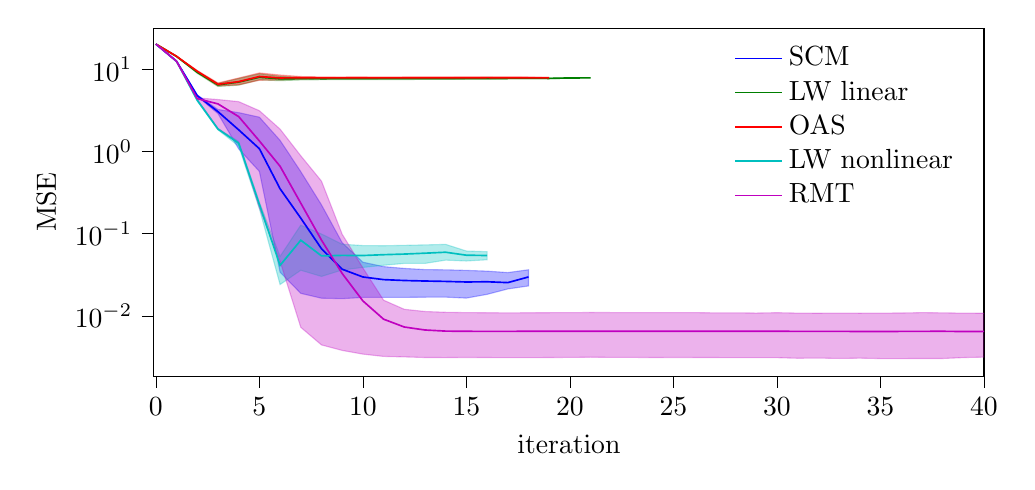
\begin{tikzpicture}

\definecolor{darkgray176}{RGB}{176,176,176}
\definecolor{darkturquoise0191191}{RGB}{0,191,191}
\definecolor{darkviolet1910191}{RGB}{191,0,191}
\definecolor{green01270}{RGB}{0,127,0}
\definecolor{lightgray204}{RGB}{204,204,204}

\begin{axis}[
width=\columnwidth,
height=6cm,
legend cell align={left},
legend style={draw=none},
log basis y={10},
tick align=outside,
tick pos=left,
unbounded coords=jump,
x grid style={darkgray176},
xlabel={iteration},
xmin=-0.1, xmax=40,
xtick style={color=black},
y grid style={darkgray176},
ylabel={MSE},
ymin=0.00185502468552686, ymax=31.5127497743851,
ymode=log,
ytick style={color=black},
ytick={0.0001,0.001,0.01,0.1,1,10,100,1000},
yticklabels={
  \(\displaystyle {10^{-4}}\),
  \(\displaystyle {10^{-3}}\),
  \(\displaystyle {10^{-2}}\),
  \(\displaystyle {10^{-1}}\),
  \(\displaystyle {10^{0}}\),
  \(\displaystyle {10^{1}}\),
  \(\displaystyle {10^{2}}\),
  \(\displaystyle {10^{3}}\)
}
]
\path [draw=blue, fill=blue, opacity=0.3]
(axis cs:0,20.2398534810237)
--(axis cs:0,20.2398534810237)
--(axis cs:1,12.4991008901501)
--(axis cs:2,4.67986487340057)
--(axis cs:3,2.88570735751221)
--(axis cs:4,1.0750914115275)
--(axis cs:5,0.572186836349737)
--(axis cs:6,0.0340889150191977)
--(axis cs:7,0.0188273555650184)
--(axis cs:8,0.0164419874210124)
--(axis cs:9,0.0162350371400239)
--(axis cs:10,0.0167964914326995)
--(axis cs:11,0.0168014503663486)
--(axis cs:12,0.0168446409133777)
--(axis cs:13,0.0169123486082042)
--(axis cs:14,0.0169407877853416)
--(axis cs:15,0.0164986880433986)
--(axis cs:16,0.0183137328383872)
--(axis cs:17,0.0213022882763265)
--(axis cs:18,0.0231730612431344)
--(axis cs:18,0.0364651895819845)
--(axis cs:18,0.0364651895819845)
--(axis cs:17,0.0336857257021297)
--(axis cs:16,0.0350642018871033)
--(axis cs:15,0.0358128830641063)
--(axis cs:14,0.0363825501407153)
--(axis cs:13,0.0366213665733975)
--(axis cs:12,0.0378601935907019)
--(axis cs:11,0.0397923813947816)
--(axis cs:10,0.0450815572720144)
--(axis cs:9,0.0777346765326108)
--(axis cs:8,0.224240910534285)
--(axis cs:7,0.568379920321504)
--(axis cs:6,1.36446320706867)
--(axis cs:5,2.61114225292828)
--(axis cs:4,2.96666407383339)
--(axis cs:3,3.23843354444121)
--(axis cs:2,4.86714647849242)
--(axis cs:1,12.5115265036264)
--(axis cs:0,20.2398534810237)
--cycle;

\path [draw=green01270, fill=green01270, opacity=0.3]
(axis cs:0,20.2398534810237)
--(axis cs:0,20.2398534810237)
--(axis cs:1,14.2599478907017)
--(axis cs:2,8.92293421911292)
--(axis cs:3,6.1727392771008)
--(axis cs:4,6.40554486542157)
--(axis cs:5,7.42443013376965)
--(axis cs:6,7.26010896478584)
--(axis cs:7,7.41689198305424)
--(axis cs:8,7.46602218392302)
--(axis cs:9,7.48854358644745)
--(axis cs:10,7.4954581032596)
--(axis cs:11,7.5028505689662)
--(axis cs:12,7.507363182864)
--(axis cs:13,7.5162932672162)
--(axis cs:14,7.54241861226889)
--(axis cs:15,7.56613856521683)
--(axis cs:16,7.59751454505805)
--(axis cs:17,7.61785348032476)
--(axis cs:18,7.66876539200264)
--(axis cs:19,7.66761969372868)
--(axis cs:20,7.83780164394383)
--(axis cs:21,7.84322945219655)
--(axis cs:21,7.84322945219655)
--(axis cs:21,7.84322945219655)
--(axis cs:20,7.83780164394383)
--(axis cs:19,7.8180478980771)
--(axis cs:18,7.8470548004764)
--(axis cs:17,7.89014391024669)
--(axis cs:16,7.93216953374447)
--(axis cs:15,7.89557136982319)
--(axis cs:14,7.88917659094287)
--(axis cs:13,7.87946089166351)
--(axis cs:12,7.87239070542018)
--(axis cs:11,7.86980578855484)
--(axis cs:10,7.87136135024433)
--(axis cs:9,7.87405411582092)
--(axis cs:8,7.89810564924487)
--(axis cs:7,7.96811631019448)
--(axis cs:6,8.22842531215863)
--(axis cs:5,8.82302440612238)
--(axis cs:4,7.71706356391931)
--(axis cs:3,6.70810783360082)
--(axis cs:2,9.42736438594104)
--(axis cs:1,14.3517189615472)
--(axis cs:0,20.2398534810237)
--cycle;

\path [draw=red, fill=red, opacity=0.3]
(axis cs:0,20.2398534810237)
--(axis cs:0,20.2398534810237)
--(axis cs:1,14.3139966160502)
--(axis cs:2,9.21615111871042)
--(axis cs:3,6.28826522177772)
--(axis cs:4,6.4607638483919)
--(axis cs:5,7.33932831048287)
--(axis cs:6,7.43045541699614)
--(axis cs:7,7.60060985993271)
--(axis cs:8,7.65965331468783)
--(axis cs:9,7.68755263502601)
--(axis cs:10,7.70095822935725)
--(axis cs:11,7.70650358000301)
--(axis cs:12,7.70969259569863)
--(axis cs:13,7.71520791319971)
--(axis cs:14,7.71005291995374)
--(axis cs:15,7.69469037671917)
--(axis cs:16,7.72066746569879)
--(axis cs:17,7.74147610339255)
--(axis cs:18,7.74720305194741)
--(axis cs:19,7.86110183514942)
--(axis cs:19,7.86110183514942)
--(axis cs:19,7.86110183514942)
--(axis cs:18,8.03046363474234)
--(axis cs:17,8.07336362358927)
--(axis cs:16,8.07152176444949)
--(axis cs:15,8.05470672175881)
--(axis cs:14,8.03590206878629)
--(axis cs:13,8.03330674999114)
--(axis cs:12,8.03146146044964)
--(axis cs:11,8.02963092443068)
--(axis cs:10,8.03178710485704)
--(axis cs:9,8.03554134008331)
--(axis cs:8,8.06057114744135)
--(axis cs:7,8.14952054630344)
--(axis cs:6,8.50892178606761)
--(axis cs:5,9.01606326956083)
--(axis cs:4,7.82275704030037)
--(axis cs:3,6.81359801310973)
--(axis cs:2,9.65580016461096)
--(axis cs:1,14.393686139361)
--(axis cs:0,20.2398534810237)
--cycle;

\path [draw=darkturquoise0191191, fill=darkturquoise0191191, opacity=0.3]
(axis cs:0,20.2398534810237)
--(axis cs:0,20.2398534810237)
--(axis cs:1,12.4784781970505)
--(axis cs:2,4.09981973543514)
--(axis cs:3,1.83332827492497)
--(axis cs:4,1.1599985629575)
--(axis cs:5,0.201724941223165)
--(axis cs:6,0.0241081639027545)
--(axis cs:7,0.0359360024873848)
--(axis cs:8,0.030243984161505)
--(axis cs:9,0.036199610161892)
--(axis cs:10,0.0389315934835895)
--(axis cs:11,0.0413464707573272)
--(axis cs:12,0.0435708928374751)
--(axis cs:13,0.0435719006694473)
--(axis cs:14,0.0477381897718535)
--(axis cs:15,0.0466000535197201)
--(axis cs:16,0.0482153871651817)
--(axis cs:16,0.0604559051427624)
--(axis cs:16,0.0604559051427624)
--(axis cs:15,0.0615969247126242)
--(axis cs:14,0.0741684571737976)
--(axis cs:13,0.073140003724847)
--(axis cs:12,0.0722002070176215)
--(axis cs:11,0.0714238245945736)
--(axis cs:10,0.0717695362631385)
--(axis cs:9,0.0745088645313488)
--(axis cs:8,0.0992153614008783)
--(axis cs:7,0.127044760635263)
--(axis cs:6,0.0531470940839386)
--(axis cs:5,0.242262874380928)
--(axis cs:4,1.32071204893679)
--(axis cs:3,1.90428574293866)
--(axis cs:2,4.28573878803838)
--(axis cs:1,12.4835223498117)
--(axis cs:0,20.2398534810237)
--cycle;

\path [draw=darkviolet1910191, fill=darkviolet1910191, opacity=0.3]
(axis cs:0,20.2398534810237)
--(axis cs:0,20.2398534810237)
--(axis cs:1,12.4815304996579)
--(axis cs:2,4.29692104067005)
--(axis cs:3,1.90155996902954)
--(axis cs:4,1.26681372977049)
--(axis cs:5,0.206228106183548)
--(axis cs:6,0.0461846470457834)
--(axis cs:7,0.00727708919056645)
--(axis cs:8,0.00444541458741207)
--(axis cs:9,0.00381202360305552)
--(axis cs:10,0.00343691573288442)
--(axis cs:11,0.00322332794787117)
--(axis cs:12,0.00318090232296529)
--(axis cs:13,0.00312367933399009)
--(axis cs:14,0.00312117489394703)
--(axis cs:15,0.00312989374616521)
--(axis cs:16,0.00312261335231817)
--(axis cs:17,0.00311808696194447)
--(axis cs:18,0.00311709030684388)
--(axis cs:19,0.00312353619356553)
--(axis cs:20,0.00313488604711713)
--(axis cs:21,0.00315329352832266)
--(axis cs:22,0.00313934940797598)
--(axis cs:23,0.00313353740579725)
--(axis cs:24,0.00312452799566201)
--(axis cs:25,0.00312799832171506)
--(axis cs:26,0.0031262828705563)
--(axis cs:27,0.00312355045698335)
--(axis cs:28,0.00311389807856909)
--(axis cs:29,0.00311179636223674)
--(axis cs:30,0.0031132516467511)
--(axis cs:31,0.00306113100705044)
--(axis cs:32,0.00307714785136851)
--(axis cs:33,0.00304409395274061)
--(axis cs:34,0.00306916600899806)
--(axis cs:35,0.0030343892705121)
--(axis cs:36,0.00303463329576796)
--(axis cs:37,0.00303716514101897)
--(axis cs:38,0.00303963641330633)
--(axis cs:39,0.00311990464829784)
--(axis cs:40,0.00315919701716498)
--(axis cs:41,0.00315481075803918)
--(axis cs:42,0.00316023365659269)
--(axis cs:43,0.00315979541369963)
--(axis cs:44,0.00315815240052234)
--(axis cs:45,0.00311601423045768)
--(axis cs:46,0.00315828436963978)
--(axis cs:47,0.00308635836975119)
--(axis cs:48,0.00302718523541201)
--(axis cs:49,0.00302621744468412)
--(axis cs:50,0.00299385710355944)
--(axis cs:51,0.00297919545472772)
--(axis cs:52,0.00297107394031857)
--(axis cs:53,0.00297133627888808)
--(axis cs:54,0.00297095822164145)
--(axis cs:55,0.00298865636882412)
--(axis cs:56,0.0030254910373631)
--(axis cs:57,0.00307812056748437)
--(axis cs:58,0.00307530738783606)
--(axis cs:59,0.00307969395554649)
--(axis cs:60,0.00305396119563578)
--(axis cs:61,0.00297822667986084)
--(axis cs:62,0.00298251090060266)
--(axis cs:63,0.00294666079372538)
--(axis cs:64,0.00293797825366746)
--(axis cs:65,0.00293110045924981)
--(axis cs:66,0.00292000593772178)
--(axis cs:67,0.00297577357142128)
--(axis cs:68,0.00304900759593814)
--(axis cs:69,0.00303448896380171)
--(axis cs:70,0.00311472908729126)
--(axis cs:71,0.00308009434546912)
--(axis cs:72,0.0031738941485334)
--(axis cs:73,0.00316213137113064)
--(axis cs:74,0.0031392442914207)
--(axis cs:75,0.00312158634586122)
--(axis cs:76,0.00308623251881578)
--(axis cs:77,0.00306276585639263)
--(axis cs:78,0.00301778453192198)
--(axis cs:79,0.00300634464739852)
--(axis cs:80,0.00303689964661294)
--(axis cs:81,0.00299010165469351)
--(axis cs:82,0.00297557328834844)
--(axis cs:83,0.00292351661043345)
--(axis cs:84,0.00291772889868639)
--(axis cs:85,0.00291317663973732)
--(axis cs:86,0.00290019255592042)
--(axis cs:87,0.00289072292912125)
--(axis cs:88,0.00288820908684555)
--(axis cs:89,0.00313418611694759)
--(axis cs:90,0.00327221463394407)
--(axis cs:91,0.00302386995065798)
--(axis cs:92,0.00293688275484942)
--(axis cs:93,0.00293657535955687)
--(axis cs:94,0.00293243051903494)
--(axis cs:95,0.00293218501106539)
--(axis cs:96,0.00293222472032092)
--(axis cs:97,0.0029240735014347)
--(axis cs:98,0.00292402022539667)
--(axis cs:99,0.00291992571793311)
--(axis cs:100,0.00291992147960144)
--(axis cs:100,0.00955380525640863)
--(axis cs:100,0.00955380525640863)
--(axis cs:99,0.00955489215838229)
--(axis cs:98,0.00940263322507785)
--(axis cs:97,0.00940323811075066)
--(axis cs:96,0.00909837936051029)
--(axis cs:95,0.00909922950577585)
--(axis cs:94,0.00909986506825843)
--(axis cs:93,0.00894822593209964)
--(axis cs:92,0.0089488909170186)
--(axis cs:91,0.00879057634604876)
--(axis cs:90,0.0087703561690065)
--(axis cs:89,0.00904091738936674)
--(axis cs:88,0.009006629689877)
--(axis cs:87,0.00898915737476655)
--(axis cs:86,0.0103585957180039)
--(axis cs:85,0.010878952828411)
--(axis cs:84,0.0108098730650499)
--(axis cs:83,0.0107406793651614)
--(axis cs:82,0.0104510623053396)
--(axis cs:81,0.0104110736968976)
--(axis cs:80,0.0103575619344988)
--(axis cs:79,0.0103176792360954)
--(axis cs:78,0.0102907652023435)
--(axis cs:77,0.0101447469023546)
--(axis cs:76,0.00999305498675339)
--(axis cs:75,0.0101004377222153)
--(axis cs:74,0.0100737106325081)
--(axis cs:73,0.0100374536787288)
--(axis cs:72,0.0104548660947733)
--(axis cs:71,0.0104014425246663)
--(axis cs:70,0.0103218089428358)
--(axis cs:69,0.0104426477531083)
--(axis cs:68,0.0104411590296086)
--(axis cs:67,0.0109032097079922)
--(axis cs:66,0.0105670088351907)
--(axis cs:65,0.0104412544774824)
--(axis cs:64,0.0104398272982936)
--(axis cs:63,0.0104376347827335)
--(axis cs:62,0.0108681184138878)
--(axis cs:61,0.0110541547616209)
--(axis cs:60,0.0109886927630625)
--(axis cs:59,0.011050961387017)
--(axis cs:58,0.0110518797915992)
--(axis cs:57,0.0110483985911132)
--(axis cs:56,0.0110443137389939)
--(axis cs:55,0.0110455109194127)
--(axis cs:54,0.0111203720448413)
--(axis cs:53,0.0110377887904728)
--(axis cs:52,0.0110093467715246)
--(axis cs:51,0.0110137852134683)
--(axis cs:50,0.0110076548206253)
--(axis cs:49,0.010901198416459)
--(axis cs:48,0.0107280294319084)
--(axis cs:47,0.0105177018130149)
--(axis cs:46,0.010728522247518)
--(axis cs:45,0.0107231085194833)
--(axis cs:44,0.0105351480002797)
--(axis cs:43,0.0105536317654251)
--(axis cs:42,0.0107298190451413)
--(axis cs:41,0.0108408837012726)
--(axis cs:40,0.0108032467705084)
--(axis cs:39,0.010809921687283)
--(axis cs:38,0.0109120857111618)
--(axis cs:37,0.0109755286035062)
--(axis cs:36,0.0108581847527652)
--(axis cs:35,0.0108382911022183)
--(axis cs:34,0.0108029852293727)
--(axis cs:33,0.0108426280616672)
--(axis cs:32,0.0107973326580203)
--(axis cs:31,0.0108269333173796)
--(axis cs:30,0.0109587831224011)
--(axis cs:29,0.0108427450601274)
--(axis cs:28,0.0109174537581877)
--(axis cs:27,0.010909501519269)
--(axis cs:26,0.0109772707902533)
--(axis cs:25,0.0109642139855248)
--(axis cs:24,0.0109722287183729)
--(axis cs:23,0.0109766944011583)
--(axis cs:22,0.011001108409474)
--(axis cs:21,0.011022850395901)
--(axis cs:20,0.010972253457087)
--(axis cs:19,0.0109582610572517)
--(axis cs:18,0.0109336629765758)
--(axis cs:17,0.010913817877843)
--(axis cs:16,0.0109404264154258)
--(axis cs:15,0.0109779777539393)
--(axis cs:14,0.0110799827527342)
--(axis cs:13,0.0113257869266612)
--(axis cs:12,0.01204825346866)
--(axis cs:11,0.0155547910137296)
--(axis cs:10,0.0383895531289296)
--(axis cs:9,0.0985245209196138)
--(axis cs:8,0.436092163077067)
--(axis cs:7,0.886243089348843)
--(axis cs:6,1.87074401777809)
--(axis cs:5,3.13139710017079)
--(axis cs:4,4.03415629435882)
--(axis cs:3,4.27694551918637)
--(axis cs:2,4.4814696808433)
--(axis cs:1,12.4887383424831)
--(axis cs:0,20.2398534810237)
--cycle;

\addplot [semithick, blue]
table {%
0 20.2398534810237
1 12.5051399454974
2 4.77410126908535
3 3.04943885239884
4 1.83287120067779
5 1.08136494028163
6 0.351841841057622
7 0.154687560247043
8 0.0657238575079157
9 0.0370101157481803
10 0.0297922684878376
11 0.0276710070689193
12 0.0269848815573062
13 0.0266064970150147
14 0.0263053266896872
15 0.0258964529322163
16 0.0260489923545703
17 0.0254406703807811
18 0.0298191254125594
19 nan
20 nan
21 nan
22 nan
23 nan
24 nan
25 nan
26 nan
27 nan
28 nan
29 nan
30 nan
31 nan
32 nan
33 nan
34 nan
35 nan
36 nan
37 nan
38 nan
39 nan
40 nan
41 nan
42 nan
43 nan
44 nan
45 nan
46 nan
47 nan
48 nan
49 nan
50 nan
51 nan
52 nan
53 nan
54 nan
55 nan
56 nan
57 nan
58 nan
59 nan
60 nan
61 nan
62 nan
63 nan
64 nan
65 nan
66 nan
67 nan
68 nan
69 nan
70 nan
71 nan
72 nan
73 nan
74 nan
75 nan
76 nan
77 nan
78 nan
79 nan
80 nan
81 nan
82 nan
83 nan
84 nan
85 nan
86 nan
87 nan
88 nan
89 nan
90 nan
91 nan
92 nan
93 nan
94 nan
95 nan
96 nan
97 nan
98 nan
99 nan
100 nan
};
\addlegendentry{SCM}
\addplot [semithick, green01270]
table {%
0 20.2398534810237
1 14.3062384942996
2 9.17838568265031
3 6.45271875007673
4 6.9885501980497
5 7.99604426499283
6 7.64274337491052
7 7.69194674005992
8 7.67595518553411
9 7.68002385451216
10 7.68133933832155
11 7.68667268900494
12 7.68968903706983
13 7.69849343761856
14 7.70386276047135
15 7.71800021187708
16 7.71719069019958
17 7.73092231348529
18 7.742443893958
19 7.72999876705468
20 7.83780164394383
21 7.84322945219655
22 nan
23 nan
24 nan
25 nan
26 nan
27 nan
28 nan
29 nan
30 nan
31 nan
32 nan
33 nan
34 nan
35 nan
36 nan
37 nan
38 nan
39 nan
40 nan
41 nan
42 nan
43 nan
44 nan
45 nan
46 nan
47 nan
48 nan
49 nan
50 nan
51 nan
52 nan
53 nan
54 nan
55 nan
56 nan
57 nan
58 nan
59 nan
60 nan
61 nan
62 nan
63 nan
64 nan
65 nan
66 nan
67 nan
68 nan
69 nan
70 nan
71 nan
72 nan
73 nan
74 nan
75 nan
76 nan
77 nan
78 nan
79 nan
80 nan
81 nan
82 nan
83 nan
84 nan
85 nan
86 nan
87 nan
88 nan
89 nan
90 nan
91 nan
92 nan
93 nan
94 nan
95 nan
96 nan
97 nan
98 nan
99 nan
100 nan
};
\addlegendentry{LW linear}
\addplot [semithick, red]
table {%
0 20.2398534810237
1 14.353491858304
2 9.43535918945406
3 6.56181131632443
4 7.05977129873939
5 8.14944380686404
6 7.83389559882885
7 7.87190138310102
8 7.85537727824357
9 7.85934714821872
10 7.86297345813823
11 7.86656906258846
12 7.86972303208463
13 7.87209341672089
14 7.87208212518206
15 7.87454693364387
16 7.89544215184673
17 7.8879900266939
18 7.8761792000927
19 7.86110183514942
20 nan
21 nan
22 nan
23 nan
24 nan
25 nan
26 nan
27 nan
28 nan
29 nan
30 nan
31 nan
32 nan
33 nan
34 nan
35 nan
36 nan
37 nan
38 nan
39 nan
40 nan
41 nan
42 nan
43 nan
44 nan
45 nan
46 nan
47 nan
48 nan
49 nan
50 nan
51 nan
52 nan
53 nan
54 nan
55 nan
56 nan
57 nan
58 nan
59 nan
60 nan
61 nan
62 nan
63 nan
64 nan
65 nan
66 nan
67 nan
68 nan
69 nan
70 nan
71 nan
72 nan
73 nan
74 nan
75 nan
76 nan
77 nan
78 nan
79 nan
80 nan
81 nan
82 nan
83 nan
84 nan
85 nan
86 nan
87 nan
88 nan
89 nan
90 nan
91 nan
92 nan
93 nan
94 nan
95 nan
96 nan
97 nan
98 nan
99 nan
100 nan
};
\addlegendentry{OAS}
\addplot [semithick, darkturquoise0191191]
table {%
0 20.2398534810237
1 12.4808416450358
2 4.19369459593088
3 1.87274583595159
4 1.2597449944868
5 0.226659333065694
6 0.0412378872500468
7 0.0834366085935366
8 0.0538065549984235
9 0.0545078387219936
10 0.0543110938282642
11 0.0555917625412838
12 0.0565698243090432
13 0.0579751230018934
14 0.0595638058127945
15 0.0548055439388746
16 0.054335646153972
17 nan
18 nan
19 nan
20 nan
21 nan
22 nan
23 nan
24 nan
25 nan
26 nan
27 nan
28 nan
29 nan
30 nan
31 nan
32 nan
33 nan
34 nan
35 nan
36 nan
37 nan
38 nan
39 nan
40 nan
41 nan
42 nan
43 nan
44 nan
45 nan
46 nan
47 nan
48 nan
49 nan
50 nan
51 nan
52 nan
53 nan
54 nan
55 nan
56 nan
57 nan
58 nan
59 nan
60 nan
61 nan
62 nan
63 nan
64 nan
65 nan
66 nan
67 nan
68 nan
69 nan
70 nan
71 nan
72 nan
73 nan
74 nan
75 nan
76 nan
77 nan
78 nan
79 nan
80 nan
81 nan
82 nan
83 nan
84 nan
85 nan
86 nan
87 nan
88 nan
89 nan
90 nan
91 nan
92 nan
93 nan
94 nan
95 nan
96 nan
97 nan
98 nan
99 nan
100 nan
};
\addlegendentry{LW nonlinear}
\addplot [semithick, darkviolet1910191]
table {%
0 20.2398534810237
1 12.4849454985754
2 4.38985446210454
3 3.78890762862372
4 2.65379303999714
5 1.34299905729867
6 0.660755526243356
7 0.235202104345185
8 0.0836089434770521
9 0.0328392212580422
10 0.0152383782743882
11 0.00913757710183963
12 0.0073395377340959
13 0.00675220293404133
14 0.00654452900770296
15 0.00650667700231331
16 0.00649972704616554
17 0.00650045950153717
18 0.00651011009723635
19 0.00651182035724732
20 0.00651498029814794
21 0.00652422463082365
22 0.0065246255535309
23 0.00652823340244216
24 0.00652616980138664
25 0.00652308185480146
26 0.0065258923633886
27 0.00652943806780616
28 0.00652794769185698
29 0.00651382601684437
30 0.00652444993547897
31 0.00649156818597608
32 0.00650268731377007
33 0.00650037242909614
34 0.00647685030935553
35 0.00646252180518286
36 0.00649253350772702
37 0.00650107703639765
38 0.00650967397111065
39 0.00647239200997801
40 0.00648936548212039
41 0.00648860942862429
42 0.00645691028912356
43 0.00641259407620643
44 0.00642376461489597
45 0.00642619024981399
46 0.00641660187011509
47 0.00635829157166954
48 0.00637922904101642
49 0.00641994781697144
50 0.00640331400792049
51 0.00639892838064257
52 0.00639726277070884
53 0.00642646508721165
54 0.00647930570277679
55 0.00646103988213072
56 0.00652885159900646
57 0.0065100467740101
58 0.00649680059326569
59 0.00649778445888401
60 0.00648581548108774
61 0.0064935016805139
62 0.00651438162523877
63 0.00642089255393926
64 0.0064567234624464
65 0.00651438819026758
66 0.00650618275830938
67 0.00658947027937457
68 0.00646931409216319
69 0.00637954492182411
70 0.00637273781463488
71 0.00644558019202535
72 0.00653223870488703
73 0.00636291729514836
74 0.00643623788301579
75 0.00645629435169436
76 0.00645505894053917
77 0.00642557033888724
78 0.00644231557724269
79 0.00652526317070573
80 0.00660584314277318
81 0.00660554048875833
82 0.00666101047039239
83 0.00673768787237661
84 0.00664137450643412
85 0.00664770617963185
86 0.00645172443400359
87 0.00635053668874626
88 0.00634099989579424
89 0.00654877109854481
90 0.00656378174847595
91 0.00660015246462207
92 0.00670149678843198
93 0.00670219898102598
94 0.0065994882485597
95 0.00659865129172461
96 0.00659665207732388
97 0.00661666634820762
98 0.00661723246562535
99 0.00674510142997628
100 0.00674541018221875
};
\addlegendentry{RMT}
\end{axis}

\end{tikzpicture}

%     \caption{MSE of the estimated mean towards true mean versus the algorithms' iterations. No value after some iteration means that stopping criterion has been attained. Monte-carlo has been done with 10000 trials. Parameters are $p=5$, $n=49$ and $K=100$.}
%     \label{fig:enter-label}
% \end{figure}

% \begin{figure*}[t]
%   \centering
%   \begin{subfigure}{0.4\textwidth}
%     % This file was created with tikzplotlib v0.10.1.
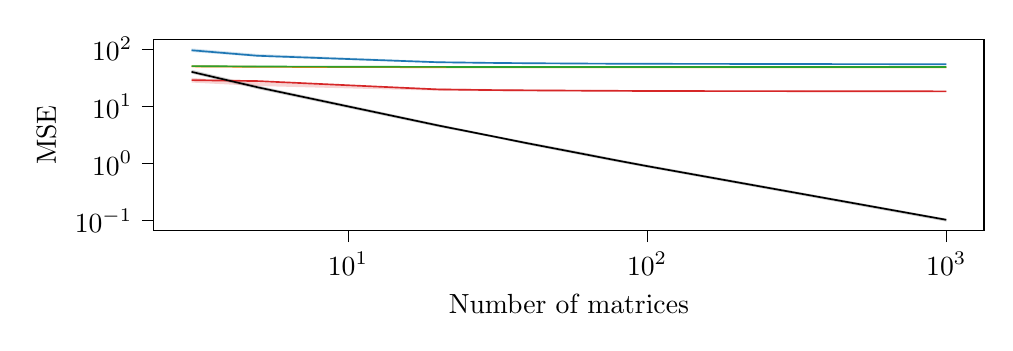
\begin{tikzpicture}

\definecolor{crimson2143940}{RGB}{214,39,40}
\definecolor{darkgray176}{RGB}{176,176,176}
\definecolor{darkorange25512714}{RGB}{255,127,14}
\definecolor{forestgreen4416044}{RGB}{44,160,44}
\definecolor{lightgray204}{RGB}{204,204,204}
\definecolor{steelblue31119180}{RGB}{31,119,180}

\begin{axis}[
width=\columnwidth,
height=4cm,
legend cell align={left},
legend style={
  fill opacity=0.8,
  draw opacity=1,
  text opacity=1,
  at={(0.03,0.03)},
  anchor=south west,
  draw=lightgray204
},
log basis x={10},
log basis y={10},
tick align=outside,
tick pos=left,
x grid style={darkgray176},
xlabel={Number of matrices},
xmin=2.2437647322819, xmax=1337.03857487278,
xmode=log,
xtick style={color=black},
xtick={0.1,1,10,100,1000,10000,100000},
xticklabels={
  \(\displaystyle {10^{-1}}\),
  \(\displaystyle {10^{0}}\),
  \(\displaystyle {10^{1}}\),
  \(\displaystyle {10^{2}}\),
  \(\displaystyle {10^{3}}\),
  \(\displaystyle {10^{4}}\),
  \(\displaystyle {10^{5}}\)
},
y grid style={darkgray176},
ylabel={MSE},
ymin=0.0676548185109966, ymax=144.054646180187,
ymode=log,
ytick style={color=black},
ytick={0.001,0.01,0.1,1,10,100,1000,10000},
yticklabels={
  \(\displaystyle {10^{-3}}\),
  \(\displaystyle {10^{-2}}\),
  \(\displaystyle {10^{-1}}\),
  \(\displaystyle {10^{0}}\),
  \(\displaystyle {10^{1}}\),
  \(\displaystyle {10^{2}}\),
  \(\displaystyle {10^{3}}\),
  \(\displaystyle {10^{4}}\)
}
]
\path [fill=steelblue31119180, fill opacity=0.2]
(axis cs:3,101.68201754882)
--(axis cs:3,88.1423662873149)
--(axis cs:5,72.3646618018412)
--(axis cs:20,56.3033594985253)
--(axis cs:30,55.2122414783319)
--(axis cs:40,54.4950492410911)
--(axis cs:60,54.3558372086263)
--(axis cs:80,53.9864569962276)
--(axis cs:100,53.7818808983528)
--(axis cs:1000,52.8842317120235)
--(axis cs:1000,54.1727833123211)
--(axis cs:1000,54.1727833123211)
--(axis cs:100,55.8890710915269)
--(axis cs:80,55.6871970646347)
--(axis cs:60,56.5784776906101)
--(axis cs:40,57.5926819637511)
--(axis cs:30,58.5444375596705)
--(axis cs:20,60.5980312773159)
--(axis cs:5,81.2598670477539)
--(axis cs:3,101.68201754882)
--cycle;

\path [fill=darkorange25512714, fill opacity=0.2]
(axis cs:3,50.9399401272127)
--(axis cs:3,47.616536256823)
--(axis cs:5,47.1612726433819)
--(axis cs:20,46.971955455793)
--(axis cs:30,47.0758081405333)
--(axis cs:40,47.0743333453457)
--(axis cs:60,46.9317172587414)
--(axis cs:80,47.0430248464519)
--(axis cs:100,47.0799238425103)
--(axis cs:1000,47.2703348549419)
--(axis cs:1000,47.4727762654529)
--(axis cs:1000,47.4727762654529)
--(axis cs:100,47.7556083668789)
--(axis cs:80,47.8016846942594)
--(axis cs:60,47.8594004527294)
--(axis cs:40,47.9763694452678)
--(axis cs:30,48.0504043908302)
--(axis cs:20,48.4899285925643)
--(axis cs:5,49.631305562104)
--(axis cs:3,50.9399401272127)
--cycle;

\path [fill=forestgreen4416044, fill opacity=0.2]
(axis cs:3,51.5543217681294)
--(axis cs:3,48.2174174363328)
--(axis cs:5,47.9435416290828)
--(axis cs:20,47.6022899376881)
--(axis cs:30,47.6905471249209)
--(axis cs:40,47.7473683750189)
--(axis cs:60,47.6137157519845)
--(axis cs:80,47.7378059813306)
--(axis cs:100,47.7700646928333)
--(axis cs:1000,47.947629843197)
--(axis cs:1000,48.1690500555604)
--(axis cs:1000,48.1690500555604)
--(axis cs:100,48.4186590813945)
--(axis cs:80,48.4745541082452)
--(axis cs:60,48.5534576983601)
--(axis cs:40,48.6446214322934)
--(axis cs:30,48.8034004170963)
--(axis cs:20,49.0483158707114)
--(axis cs:5,50.2587948881218)
--(axis cs:3,51.5543217681294)
--cycle;

\path [fill=crimson2143940, fill opacity=0.2]
(axis cs:3,31.0620901659341)
--(axis cs:3,25.7814354065144)
--(axis cs:5,22.4151766483135)
--(axis cs:20,18.5613287460143)
--(axis cs:30,18.2068668295756)
--(axis cs:40,18.0053951577646)
--(axis cs:60,18.0719911571276)
--(axis cs:80,18.0540496547627)
--(axis cs:100,17.8175733279627)
--(axis cs:1000,17.9286725829367)
--(axis cs:1000,18.2797926395433)
--(axis cs:1000,18.2797926395433)
--(axis cs:100,18.8026404764028)
--(axis cs:80,18.9858881503917)
--(axis cs:60,19.1340577061154)
--(axis cs:40,19.5820574055868)
--(axis cs:30,19.8302337288776)
--(axis cs:20,20.3582799108111)
--(axis cs:5,26.0822272030139)
--(axis cs:3,31.0620901659341)
--cycle;

\path [fill=black, fill opacity=0.2]
(axis cs:3,43.0134914235546)
--(axis cs:3,37.0492981565219)
--(axis cs:5,19.756909188043)
--(axis cs:20,4.31132775896778)
--(axis cs:30,2.86976889713881)
--(axis cs:40,2.09763141896607)
--(axis cs:60,1.39543284162807)
--(axis cs:80,1.04403044418553)
--(axis cs:100,0.842579436435285)
--(axis cs:1000,0.0958477337284056)
--(axis cs:1000,0.108031285268237)
--(axis cs:1000,0.108031285268237)
--(axis cs:100,0.944582470496131)
--(axis cs:80,1.17145085610537)
--(axis cs:60,1.5782483886311)
--(axis cs:40,2.3540862718306)
--(axis cs:30,3.154578637464)
--(axis cs:20,4.84674945358772)
--(axis cs:5,22.7658116599057)
--(axis cs:3,43.0134914235546)
--cycle;

\addplot [semithick, steelblue31119180]
table {%
3 94.5157592925942
5 75.6586882309294
20 58.353278559489
30 56.8241460264265
40 56.0826200766897
60 55.3597906632788
80 54.9424181564402
100 54.8161336747953
1000 53.7897210817627
};
\addlegendentry{SCM}
\addplot [semithick, darkorange25512714]
table {%
3 49.3613074737249
5 48.483748351865
20 47.6761402802835
30 47.5720824300155
40 47.5095728646513
60 47.4147988906565
80 47.4285959048943
100 47.4332061562883
1000 47.3704802116759
};
\addlegendentry{LW linear}
\addplot [semithick, forestgreen4416044]
table {%
3 49.9280772828501
5 49.1190938760236
20 48.3424993688959
30 48.2593143364372
40 48.1882416288635
60 48.097836189495
80 48.0973273595286
100 48.1184165931483
1000 48.0624897968217
};
\addlegendentry{OAS}
\addplot [semithick, crimson2143940]
table {%
3 28.4039460003532
5 27.3315303143067
20 19.5467182255244
30 19.0379044881684
40 18.8116447240747
60 18.5874615737571
80 18.4667134698607
100 18.3262967067618
1000 18.0866390671002
};
\addlegendentry{LW nonlinear}
\addplot [semithick, black]
table {%
3 39.6510294255462
5 21.2484674975276
20 4.58847604525462
30 3.01179037254277
40 2.22860231661461
60 1.48283062300453
80 1.1099362145875
100 0.892233532399277
1000 0.102898126015732
};
\addlegendentry{RMT}

\legend{};
\end{axis}

\end{tikzpicture}

%     \caption{$p=5$, $n=7$}
%     \label{fig:subfiga}
%   \end{subfigure}
%   \begin{subfigure}{0.4\textwidth}
%     % This file was created with tikzplotlib v0.10.1.
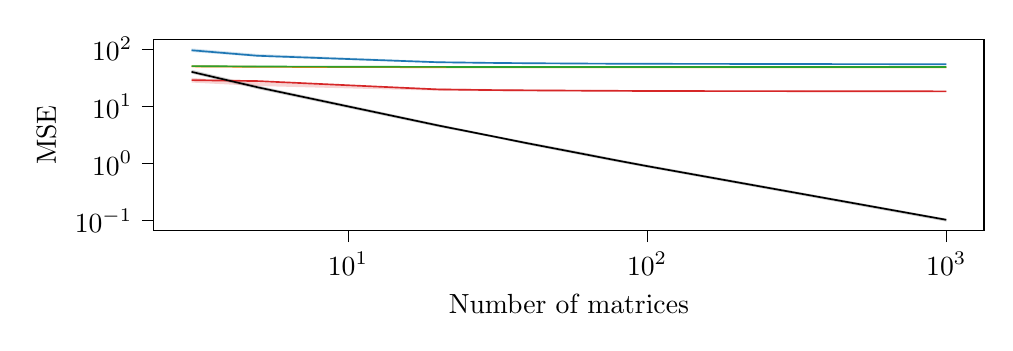
\begin{tikzpicture}

\definecolor{crimson2143940}{RGB}{214,39,40}
\definecolor{darkgray176}{RGB}{176,176,176}
\definecolor{darkorange25512714}{RGB}{255,127,14}
\definecolor{forestgreen4416044}{RGB}{44,160,44}
\definecolor{lightgray204}{RGB}{204,204,204}
\definecolor{steelblue31119180}{RGB}{31,119,180}

\begin{axis}[
width=\columnwidth,
height=4cm,
legend cell align={left},
legend style={
  fill opacity=0.8,
  draw opacity=1,
  text opacity=1,
  at={(0.03,0.03)},
  anchor=south west,
  draw=lightgray204
},
log basis x={10},
log basis y={10},
tick align=outside,
tick pos=left,
x grid style={darkgray176},
xlabel={Number of matrices},
xmin=2.2437647322819, xmax=1337.03857487278,
xmode=log,
xtick style={color=black},
xtick={0.1,1,10,100,1000,10000,100000},
xticklabels={
  \(\displaystyle {10^{-1}}\),
  \(\displaystyle {10^{0}}\),
  \(\displaystyle {10^{1}}\),
  \(\displaystyle {10^{2}}\),
  \(\displaystyle {10^{3}}\),
  \(\displaystyle {10^{4}}\),
  \(\displaystyle {10^{5}}\)
},
y grid style={darkgray176},
ylabel={MSE},
ymin=0.0676548185109966, ymax=144.054646180187,
ymode=log,
ytick style={color=black},
ytick={0.001,0.01,0.1,1,10,100,1000,10000},
yticklabels={
  \(\displaystyle {10^{-3}}\),
  \(\displaystyle {10^{-2}}\),
  \(\displaystyle {10^{-1}}\),
  \(\displaystyle {10^{0}}\),
  \(\displaystyle {10^{1}}\),
  \(\displaystyle {10^{2}}\),
  \(\displaystyle {10^{3}}\),
  \(\displaystyle {10^{4}}\)
}
]
\path [fill=steelblue31119180, fill opacity=0.2]
(axis cs:3,101.68201754882)
--(axis cs:3,88.1423662873149)
--(axis cs:5,72.3646618018412)
--(axis cs:20,56.3033594985253)
--(axis cs:30,55.2122414783319)
--(axis cs:40,54.4950492410911)
--(axis cs:60,54.3558372086263)
--(axis cs:80,53.9864569962276)
--(axis cs:100,53.7818808983528)
--(axis cs:1000,52.8842317120235)
--(axis cs:1000,54.1727833123211)
--(axis cs:1000,54.1727833123211)
--(axis cs:100,55.8890710915269)
--(axis cs:80,55.6871970646347)
--(axis cs:60,56.5784776906101)
--(axis cs:40,57.5926819637511)
--(axis cs:30,58.5444375596705)
--(axis cs:20,60.5980312773159)
--(axis cs:5,81.2598670477539)
--(axis cs:3,101.68201754882)
--cycle;

\path [fill=darkorange25512714, fill opacity=0.2]
(axis cs:3,50.9399401272127)
--(axis cs:3,47.616536256823)
--(axis cs:5,47.1612726433819)
--(axis cs:20,46.971955455793)
--(axis cs:30,47.0758081405333)
--(axis cs:40,47.0743333453457)
--(axis cs:60,46.9317172587414)
--(axis cs:80,47.0430248464519)
--(axis cs:100,47.0799238425103)
--(axis cs:1000,47.2703348549419)
--(axis cs:1000,47.4727762654529)
--(axis cs:1000,47.4727762654529)
--(axis cs:100,47.7556083668789)
--(axis cs:80,47.8016846942594)
--(axis cs:60,47.8594004527294)
--(axis cs:40,47.9763694452678)
--(axis cs:30,48.0504043908302)
--(axis cs:20,48.4899285925643)
--(axis cs:5,49.631305562104)
--(axis cs:3,50.9399401272127)
--cycle;

\path [fill=forestgreen4416044, fill opacity=0.2]
(axis cs:3,51.5543217681294)
--(axis cs:3,48.2174174363328)
--(axis cs:5,47.9435416290828)
--(axis cs:20,47.6022899376881)
--(axis cs:30,47.6905471249209)
--(axis cs:40,47.7473683750189)
--(axis cs:60,47.6137157519845)
--(axis cs:80,47.7378059813306)
--(axis cs:100,47.7700646928333)
--(axis cs:1000,47.947629843197)
--(axis cs:1000,48.1690500555604)
--(axis cs:1000,48.1690500555604)
--(axis cs:100,48.4186590813945)
--(axis cs:80,48.4745541082452)
--(axis cs:60,48.5534576983601)
--(axis cs:40,48.6446214322934)
--(axis cs:30,48.8034004170963)
--(axis cs:20,49.0483158707114)
--(axis cs:5,50.2587948881218)
--(axis cs:3,51.5543217681294)
--cycle;

\path [fill=crimson2143940, fill opacity=0.2]
(axis cs:3,31.0620901659341)
--(axis cs:3,25.7814354065144)
--(axis cs:5,22.4151766483135)
--(axis cs:20,18.5613287460143)
--(axis cs:30,18.2068668295756)
--(axis cs:40,18.0053951577646)
--(axis cs:60,18.0719911571276)
--(axis cs:80,18.0540496547627)
--(axis cs:100,17.8175733279627)
--(axis cs:1000,17.9286725829367)
--(axis cs:1000,18.2797926395433)
--(axis cs:1000,18.2797926395433)
--(axis cs:100,18.8026404764028)
--(axis cs:80,18.9858881503917)
--(axis cs:60,19.1340577061154)
--(axis cs:40,19.5820574055868)
--(axis cs:30,19.8302337288776)
--(axis cs:20,20.3582799108111)
--(axis cs:5,26.0822272030139)
--(axis cs:3,31.0620901659341)
--cycle;

\path [fill=black, fill opacity=0.2]
(axis cs:3,43.0134914235546)
--(axis cs:3,37.0492981565219)
--(axis cs:5,19.756909188043)
--(axis cs:20,4.31132775896778)
--(axis cs:30,2.86976889713881)
--(axis cs:40,2.09763141896607)
--(axis cs:60,1.39543284162807)
--(axis cs:80,1.04403044418553)
--(axis cs:100,0.842579436435285)
--(axis cs:1000,0.0958477337284056)
--(axis cs:1000,0.108031285268237)
--(axis cs:1000,0.108031285268237)
--(axis cs:100,0.944582470496131)
--(axis cs:80,1.17145085610537)
--(axis cs:60,1.5782483886311)
--(axis cs:40,2.3540862718306)
--(axis cs:30,3.154578637464)
--(axis cs:20,4.84674945358772)
--(axis cs:5,22.7658116599057)
--(axis cs:3,43.0134914235546)
--cycle;

\addplot [semithick, steelblue31119180]
table {%
3 94.5157592925942
5 75.6586882309294
20 58.353278559489
30 56.8241460264265
40 56.0826200766897
60 55.3597906632788
80 54.9424181564402
100 54.8161336747953
1000 53.7897210817627
};
\addlegendentry{SCM}
\addplot [semithick, darkorange25512714]
table {%
3 49.3613074737249
5 48.483748351865
20 47.6761402802835
30 47.5720824300155
40 47.5095728646513
60 47.4147988906565
80 47.4285959048943
100 47.4332061562883
1000 47.3704802116759
};
\addlegendentry{LW linear}
\addplot [semithick, forestgreen4416044]
table {%
3 49.9280772828501
5 49.1190938760236
20 48.3424993688959
30 48.2593143364372
40 48.1882416288635
60 48.097836189495
80 48.0973273595286
100 48.1184165931483
1000 48.0624897968217
};
\addlegendentry{OAS}
\addplot [semithick, crimson2143940]
table {%
3 28.4039460003532
5 27.3315303143067
20 19.5467182255244
30 19.0379044881684
40 18.8116447240747
60 18.5874615737571
80 18.4667134698607
100 18.3262967067618
1000 18.0866390671002
};
\addlegendentry{LW nonlinear}
\addplot [semithick, black]
table {%
3 39.6510294255462
5 21.2484674975276
20 4.58847604525462
30 3.01179037254277
40 2.22860231661461
60 1.48283062300453
80 1.1099362145875
100 0.892233532399277
1000 0.102898126015732
};
\addlegendentry{RMT}

\legend{};
\end{axis}

\end{tikzpicture}

%     \caption{$p=5$, $n=25$}
%     \label{fig:subfigb}
%   \end{subfigure}
%   \begin{subfigure}{0.4\textwidth}
%     % This file was created with tikzplotlib v0.10.1.
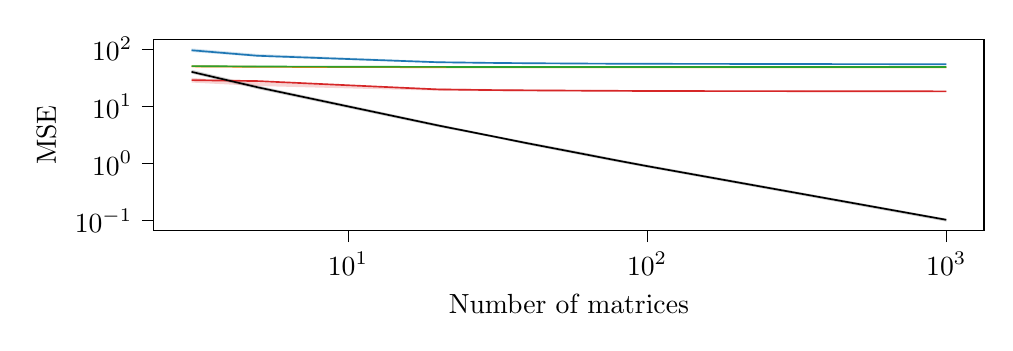
\begin{tikzpicture}

\definecolor{crimson2143940}{RGB}{214,39,40}
\definecolor{darkgray176}{RGB}{176,176,176}
\definecolor{darkorange25512714}{RGB}{255,127,14}
\definecolor{forestgreen4416044}{RGB}{44,160,44}
\definecolor{lightgray204}{RGB}{204,204,204}
\definecolor{steelblue31119180}{RGB}{31,119,180}

\begin{axis}[
width=\columnwidth,
height=4cm,
legend cell align={left},
legend style={
  fill opacity=0.8,
  draw opacity=1,
  text opacity=1,
  at={(0.03,0.03)},
  anchor=south west,
  draw=lightgray204
},
log basis x={10},
log basis y={10},
tick align=outside,
tick pos=left,
x grid style={darkgray176},
xlabel={Number of matrices},
xmin=2.2437647322819, xmax=1337.03857487278,
xmode=log,
xtick style={color=black},
xtick={0.1,1,10,100,1000,10000,100000},
xticklabels={
  \(\displaystyle {10^{-1}}\),
  \(\displaystyle {10^{0}}\),
  \(\displaystyle {10^{1}}\),
  \(\displaystyle {10^{2}}\),
  \(\displaystyle {10^{3}}\),
  \(\displaystyle {10^{4}}\),
  \(\displaystyle {10^{5}}\)
},
y grid style={darkgray176},
ylabel={MSE},
ymin=0.0676548185109966, ymax=144.054646180187,
ymode=log,
ytick style={color=black},
ytick={0.001,0.01,0.1,1,10,100,1000,10000},
yticklabels={
  \(\displaystyle {10^{-3}}\),
  \(\displaystyle {10^{-2}}\),
  \(\displaystyle {10^{-1}}\),
  \(\displaystyle {10^{0}}\),
  \(\displaystyle {10^{1}}\),
  \(\displaystyle {10^{2}}\),
  \(\displaystyle {10^{3}}\),
  \(\displaystyle {10^{4}}\)
}
]
\path [fill=steelblue31119180, fill opacity=0.2]
(axis cs:3,101.68201754882)
--(axis cs:3,88.1423662873149)
--(axis cs:5,72.3646618018412)
--(axis cs:20,56.3033594985253)
--(axis cs:30,55.2122414783319)
--(axis cs:40,54.4950492410911)
--(axis cs:60,54.3558372086263)
--(axis cs:80,53.9864569962276)
--(axis cs:100,53.7818808983528)
--(axis cs:1000,52.8842317120235)
--(axis cs:1000,54.1727833123211)
--(axis cs:1000,54.1727833123211)
--(axis cs:100,55.8890710915269)
--(axis cs:80,55.6871970646347)
--(axis cs:60,56.5784776906101)
--(axis cs:40,57.5926819637511)
--(axis cs:30,58.5444375596705)
--(axis cs:20,60.5980312773159)
--(axis cs:5,81.2598670477539)
--(axis cs:3,101.68201754882)
--cycle;

\path [fill=darkorange25512714, fill opacity=0.2]
(axis cs:3,50.9399401272127)
--(axis cs:3,47.616536256823)
--(axis cs:5,47.1612726433819)
--(axis cs:20,46.971955455793)
--(axis cs:30,47.0758081405333)
--(axis cs:40,47.0743333453457)
--(axis cs:60,46.9317172587414)
--(axis cs:80,47.0430248464519)
--(axis cs:100,47.0799238425103)
--(axis cs:1000,47.2703348549419)
--(axis cs:1000,47.4727762654529)
--(axis cs:1000,47.4727762654529)
--(axis cs:100,47.7556083668789)
--(axis cs:80,47.8016846942594)
--(axis cs:60,47.8594004527294)
--(axis cs:40,47.9763694452678)
--(axis cs:30,48.0504043908302)
--(axis cs:20,48.4899285925643)
--(axis cs:5,49.631305562104)
--(axis cs:3,50.9399401272127)
--cycle;

\path [fill=forestgreen4416044, fill opacity=0.2]
(axis cs:3,51.5543217681294)
--(axis cs:3,48.2174174363328)
--(axis cs:5,47.9435416290828)
--(axis cs:20,47.6022899376881)
--(axis cs:30,47.6905471249209)
--(axis cs:40,47.7473683750189)
--(axis cs:60,47.6137157519845)
--(axis cs:80,47.7378059813306)
--(axis cs:100,47.7700646928333)
--(axis cs:1000,47.947629843197)
--(axis cs:1000,48.1690500555604)
--(axis cs:1000,48.1690500555604)
--(axis cs:100,48.4186590813945)
--(axis cs:80,48.4745541082452)
--(axis cs:60,48.5534576983601)
--(axis cs:40,48.6446214322934)
--(axis cs:30,48.8034004170963)
--(axis cs:20,49.0483158707114)
--(axis cs:5,50.2587948881218)
--(axis cs:3,51.5543217681294)
--cycle;

\path [fill=crimson2143940, fill opacity=0.2]
(axis cs:3,31.0620901659341)
--(axis cs:3,25.7814354065144)
--(axis cs:5,22.4151766483135)
--(axis cs:20,18.5613287460143)
--(axis cs:30,18.2068668295756)
--(axis cs:40,18.0053951577646)
--(axis cs:60,18.0719911571276)
--(axis cs:80,18.0540496547627)
--(axis cs:100,17.8175733279627)
--(axis cs:1000,17.9286725829367)
--(axis cs:1000,18.2797926395433)
--(axis cs:1000,18.2797926395433)
--(axis cs:100,18.8026404764028)
--(axis cs:80,18.9858881503917)
--(axis cs:60,19.1340577061154)
--(axis cs:40,19.5820574055868)
--(axis cs:30,19.8302337288776)
--(axis cs:20,20.3582799108111)
--(axis cs:5,26.0822272030139)
--(axis cs:3,31.0620901659341)
--cycle;

\path [fill=black, fill opacity=0.2]
(axis cs:3,43.0134914235546)
--(axis cs:3,37.0492981565219)
--(axis cs:5,19.756909188043)
--(axis cs:20,4.31132775896778)
--(axis cs:30,2.86976889713881)
--(axis cs:40,2.09763141896607)
--(axis cs:60,1.39543284162807)
--(axis cs:80,1.04403044418553)
--(axis cs:100,0.842579436435285)
--(axis cs:1000,0.0958477337284056)
--(axis cs:1000,0.108031285268237)
--(axis cs:1000,0.108031285268237)
--(axis cs:100,0.944582470496131)
--(axis cs:80,1.17145085610537)
--(axis cs:60,1.5782483886311)
--(axis cs:40,2.3540862718306)
--(axis cs:30,3.154578637464)
--(axis cs:20,4.84674945358772)
--(axis cs:5,22.7658116599057)
--(axis cs:3,43.0134914235546)
--cycle;

\addplot [semithick, steelblue31119180]
table {%
3 94.5157592925942
5 75.6586882309294
20 58.353278559489
30 56.8241460264265
40 56.0826200766897
60 55.3597906632788
80 54.9424181564402
100 54.8161336747953
1000 53.7897210817627
};
\addlegendentry{SCM}
\addplot [semithick, darkorange25512714]
table {%
3 49.3613074737249
5 48.483748351865
20 47.6761402802835
30 47.5720824300155
40 47.5095728646513
60 47.4147988906565
80 47.4285959048943
100 47.4332061562883
1000 47.3704802116759
};
\addlegendentry{LW linear}
\addplot [semithick, forestgreen4416044]
table {%
3 49.9280772828501
5 49.1190938760236
20 48.3424993688959
30 48.2593143364372
40 48.1882416288635
60 48.097836189495
80 48.0973273595286
100 48.1184165931483
1000 48.0624897968217
};
\addlegendentry{OAS}
\addplot [semithick, crimson2143940]
table {%
3 28.4039460003532
5 27.3315303143067
20 19.5467182255244
30 19.0379044881684
40 18.8116447240747
60 18.5874615737571
80 18.4667134698607
100 18.3262967067618
1000 18.0866390671002
};
\addlegendentry{LW nonlinear}
\addplot [semithick, black]
table {%
3 39.6510294255462
5 21.2484674975276
20 4.58847604525462
30 3.01179037254277
40 2.22860231661461
60 1.48283062300453
80 1.1099362145875
100 0.892233532399277
1000 0.102898126015732
};
\addlegendentry{RMT}

\legend{};
\end{axis}

\end{tikzpicture}

%     \caption{$p=64$, $n=66$}
%     \label{fig:subfiga}
%   \end{subfigure}
%   \begin{subfigure}{0.4\textwidth}
%     % This file was created with tikzplotlib v0.10.1.
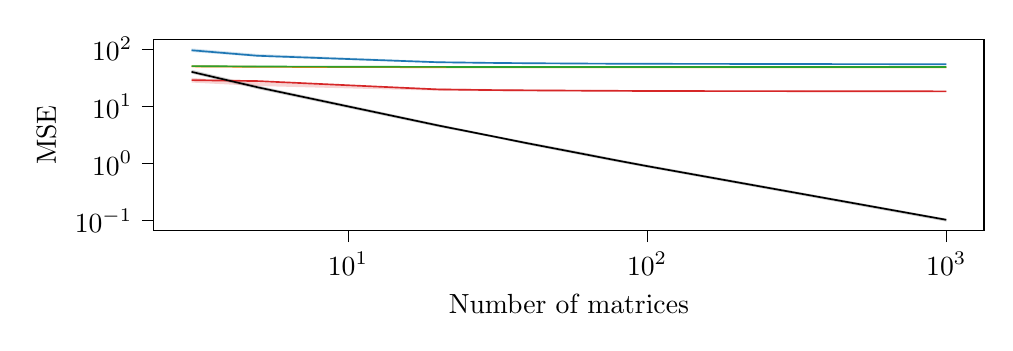
\begin{tikzpicture}

\definecolor{crimson2143940}{RGB}{214,39,40}
\definecolor{darkgray176}{RGB}{176,176,176}
\definecolor{darkorange25512714}{RGB}{255,127,14}
\definecolor{forestgreen4416044}{RGB}{44,160,44}
\definecolor{lightgray204}{RGB}{204,204,204}
\definecolor{steelblue31119180}{RGB}{31,119,180}

\begin{axis}[
width=\columnwidth,
height=4cm,
legend cell align={left},
legend style={
  fill opacity=0.8,
  draw opacity=1,
  text opacity=1,
  at={(0.03,0.03)},
  anchor=south west,
  draw=lightgray204
},
log basis x={10},
log basis y={10},
tick align=outside,
tick pos=left,
x grid style={darkgray176},
xlabel={Number of matrices},
xmin=2.2437647322819, xmax=1337.03857487278,
xmode=log,
xtick style={color=black},
xtick={0.1,1,10,100,1000,10000,100000},
xticklabels={
  \(\displaystyle {10^{-1}}\),
  \(\displaystyle {10^{0}}\),
  \(\displaystyle {10^{1}}\),
  \(\displaystyle {10^{2}}\),
  \(\displaystyle {10^{3}}\),
  \(\displaystyle {10^{4}}\),
  \(\displaystyle {10^{5}}\)
},
y grid style={darkgray176},
ylabel={MSE},
ymin=0.0676548185109966, ymax=144.054646180187,
ymode=log,
ytick style={color=black},
ytick={0.001,0.01,0.1,1,10,100,1000,10000},
yticklabels={
  \(\displaystyle {10^{-3}}\),
  \(\displaystyle {10^{-2}}\),
  \(\displaystyle {10^{-1}}\),
  \(\displaystyle {10^{0}}\),
  \(\displaystyle {10^{1}}\),
  \(\displaystyle {10^{2}}\),
  \(\displaystyle {10^{3}}\),
  \(\displaystyle {10^{4}}\)
}
]
\path [fill=steelblue31119180, fill opacity=0.2]
(axis cs:3,101.68201754882)
--(axis cs:3,88.1423662873149)
--(axis cs:5,72.3646618018412)
--(axis cs:20,56.3033594985253)
--(axis cs:30,55.2122414783319)
--(axis cs:40,54.4950492410911)
--(axis cs:60,54.3558372086263)
--(axis cs:80,53.9864569962276)
--(axis cs:100,53.7818808983528)
--(axis cs:1000,52.8842317120235)
--(axis cs:1000,54.1727833123211)
--(axis cs:1000,54.1727833123211)
--(axis cs:100,55.8890710915269)
--(axis cs:80,55.6871970646347)
--(axis cs:60,56.5784776906101)
--(axis cs:40,57.5926819637511)
--(axis cs:30,58.5444375596705)
--(axis cs:20,60.5980312773159)
--(axis cs:5,81.2598670477539)
--(axis cs:3,101.68201754882)
--cycle;

\path [fill=darkorange25512714, fill opacity=0.2]
(axis cs:3,50.9399401272127)
--(axis cs:3,47.616536256823)
--(axis cs:5,47.1612726433819)
--(axis cs:20,46.971955455793)
--(axis cs:30,47.0758081405333)
--(axis cs:40,47.0743333453457)
--(axis cs:60,46.9317172587414)
--(axis cs:80,47.0430248464519)
--(axis cs:100,47.0799238425103)
--(axis cs:1000,47.2703348549419)
--(axis cs:1000,47.4727762654529)
--(axis cs:1000,47.4727762654529)
--(axis cs:100,47.7556083668789)
--(axis cs:80,47.8016846942594)
--(axis cs:60,47.8594004527294)
--(axis cs:40,47.9763694452678)
--(axis cs:30,48.0504043908302)
--(axis cs:20,48.4899285925643)
--(axis cs:5,49.631305562104)
--(axis cs:3,50.9399401272127)
--cycle;

\path [fill=forestgreen4416044, fill opacity=0.2]
(axis cs:3,51.5543217681294)
--(axis cs:3,48.2174174363328)
--(axis cs:5,47.9435416290828)
--(axis cs:20,47.6022899376881)
--(axis cs:30,47.6905471249209)
--(axis cs:40,47.7473683750189)
--(axis cs:60,47.6137157519845)
--(axis cs:80,47.7378059813306)
--(axis cs:100,47.7700646928333)
--(axis cs:1000,47.947629843197)
--(axis cs:1000,48.1690500555604)
--(axis cs:1000,48.1690500555604)
--(axis cs:100,48.4186590813945)
--(axis cs:80,48.4745541082452)
--(axis cs:60,48.5534576983601)
--(axis cs:40,48.6446214322934)
--(axis cs:30,48.8034004170963)
--(axis cs:20,49.0483158707114)
--(axis cs:5,50.2587948881218)
--(axis cs:3,51.5543217681294)
--cycle;

\path [fill=crimson2143940, fill opacity=0.2]
(axis cs:3,31.0620901659341)
--(axis cs:3,25.7814354065144)
--(axis cs:5,22.4151766483135)
--(axis cs:20,18.5613287460143)
--(axis cs:30,18.2068668295756)
--(axis cs:40,18.0053951577646)
--(axis cs:60,18.0719911571276)
--(axis cs:80,18.0540496547627)
--(axis cs:100,17.8175733279627)
--(axis cs:1000,17.9286725829367)
--(axis cs:1000,18.2797926395433)
--(axis cs:1000,18.2797926395433)
--(axis cs:100,18.8026404764028)
--(axis cs:80,18.9858881503917)
--(axis cs:60,19.1340577061154)
--(axis cs:40,19.5820574055868)
--(axis cs:30,19.8302337288776)
--(axis cs:20,20.3582799108111)
--(axis cs:5,26.0822272030139)
--(axis cs:3,31.0620901659341)
--cycle;

\path [fill=black, fill opacity=0.2]
(axis cs:3,43.0134914235546)
--(axis cs:3,37.0492981565219)
--(axis cs:5,19.756909188043)
--(axis cs:20,4.31132775896778)
--(axis cs:30,2.86976889713881)
--(axis cs:40,2.09763141896607)
--(axis cs:60,1.39543284162807)
--(axis cs:80,1.04403044418553)
--(axis cs:100,0.842579436435285)
--(axis cs:1000,0.0958477337284056)
--(axis cs:1000,0.108031285268237)
--(axis cs:1000,0.108031285268237)
--(axis cs:100,0.944582470496131)
--(axis cs:80,1.17145085610537)
--(axis cs:60,1.5782483886311)
--(axis cs:40,2.3540862718306)
--(axis cs:30,3.154578637464)
--(axis cs:20,4.84674945358772)
--(axis cs:5,22.7658116599057)
--(axis cs:3,43.0134914235546)
--cycle;

\addplot [semithick, steelblue31119180]
table {%
3 94.5157592925942
5 75.6586882309294
20 58.353278559489
30 56.8241460264265
40 56.0826200766897
60 55.3597906632788
80 54.9424181564402
100 54.8161336747953
1000 53.7897210817627
};
\addlegendentry{SCM}
\addplot [semithick, darkorange25512714]
table {%
3 49.3613074737249
5 48.483748351865
20 47.6761402802835
30 47.5720824300155
40 47.5095728646513
60 47.4147988906565
80 47.4285959048943
100 47.4332061562883
1000 47.3704802116759
};
\addlegendentry{LW linear}
\addplot [semithick, forestgreen4416044]
table {%
3 49.9280772828501
5 49.1190938760236
20 48.3424993688959
30 48.2593143364372
40 48.1882416288635
60 48.097836189495
80 48.0973273595286
100 48.1184165931483
1000 48.0624897968217
};
\addlegendentry{OAS}
\addplot [semithick, crimson2143940]
table {%
3 28.4039460003532
5 27.3315303143067
20 19.5467182255244
30 19.0379044881684
40 18.8116447240747
60 18.5874615737571
80 18.4667134698607
100 18.3262967067618
1000 18.0866390671002
};
\addlegendentry{LW nonlinear}
\addplot [semithick, black]
table {%
3 39.6510294255462
5 21.2484674975276
20 4.58847604525462
30 3.01179037254277
40 2.22860231661461
60 1.48283062300453
80 1.1099362145875
100 0.892233532399277
1000 0.102898126015732
};
\addlegendentry{RMT}

\legend{};
\end{axis}

\end{tikzpicture}

%     \caption{$p=64$, $n=128$}
%     \label{fig:subfigb}
%   \end{subfigure}
%   \begin{subfigure}{0.4\textwidth}
%     % This file was created with tikzplotlib v0.10.1.
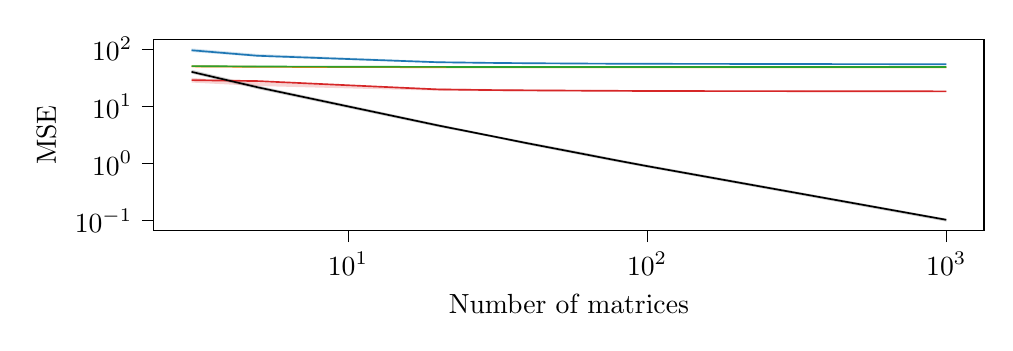
\begin{tikzpicture}

\definecolor{crimson2143940}{RGB}{214,39,40}
\definecolor{darkgray176}{RGB}{176,176,176}
\definecolor{darkorange25512714}{RGB}{255,127,14}
\definecolor{forestgreen4416044}{RGB}{44,160,44}
\definecolor{lightgray204}{RGB}{204,204,204}
\definecolor{steelblue31119180}{RGB}{31,119,180}

\begin{axis}[
width=\columnwidth,
height=4cm,
legend cell align={left},
legend style={
  fill opacity=0.8,
  draw opacity=1,
  text opacity=1,
  at={(0.03,0.03)},
  anchor=south west,
  draw=lightgray204
},
log basis x={10},
log basis y={10},
tick align=outside,
tick pos=left,
x grid style={darkgray176},
xlabel={Number of matrices},
xmin=2.2437647322819, xmax=1337.03857487278,
xmode=log,
xtick style={color=black},
xtick={0.1,1,10,100,1000,10000,100000},
xticklabels={
  \(\displaystyle {10^{-1}}\),
  \(\displaystyle {10^{0}}\),
  \(\displaystyle {10^{1}}\),
  \(\displaystyle {10^{2}}\),
  \(\displaystyle {10^{3}}\),
  \(\displaystyle {10^{4}}\),
  \(\displaystyle {10^{5}}\)
},
y grid style={darkgray176},
ylabel={MSE},
ymin=0.0676548185109966, ymax=144.054646180187,
ymode=log,
ytick style={color=black},
ytick={0.001,0.01,0.1,1,10,100,1000,10000},
yticklabels={
  \(\displaystyle {10^{-3}}\),
  \(\displaystyle {10^{-2}}\),
  \(\displaystyle {10^{-1}}\),
  \(\displaystyle {10^{0}}\),
  \(\displaystyle {10^{1}}\),
  \(\displaystyle {10^{2}}\),
  \(\displaystyle {10^{3}}\),
  \(\displaystyle {10^{4}}\)
}
]
\path [fill=steelblue31119180, fill opacity=0.2]
(axis cs:3,101.68201754882)
--(axis cs:3,88.1423662873149)
--(axis cs:5,72.3646618018412)
--(axis cs:20,56.3033594985253)
--(axis cs:30,55.2122414783319)
--(axis cs:40,54.4950492410911)
--(axis cs:60,54.3558372086263)
--(axis cs:80,53.9864569962276)
--(axis cs:100,53.7818808983528)
--(axis cs:1000,52.8842317120235)
--(axis cs:1000,54.1727833123211)
--(axis cs:1000,54.1727833123211)
--(axis cs:100,55.8890710915269)
--(axis cs:80,55.6871970646347)
--(axis cs:60,56.5784776906101)
--(axis cs:40,57.5926819637511)
--(axis cs:30,58.5444375596705)
--(axis cs:20,60.5980312773159)
--(axis cs:5,81.2598670477539)
--(axis cs:3,101.68201754882)
--cycle;

\path [fill=darkorange25512714, fill opacity=0.2]
(axis cs:3,50.9399401272127)
--(axis cs:3,47.616536256823)
--(axis cs:5,47.1612726433819)
--(axis cs:20,46.971955455793)
--(axis cs:30,47.0758081405333)
--(axis cs:40,47.0743333453457)
--(axis cs:60,46.9317172587414)
--(axis cs:80,47.0430248464519)
--(axis cs:100,47.0799238425103)
--(axis cs:1000,47.2703348549419)
--(axis cs:1000,47.4727762654529)
--(axis cs:1000,47.4727762654529)
--(axis cs:100,47.7556083668789)
--(axis cs:80,47.8016846942594)
--(axis cs:60,47.8594004527294)
--(axis cs:40,47.9763694452678)
--(axis cs:30,48.0504043908302)
--(axis cs:20,48.4899285925643)
--(axis cs:5,49.631305562104)
--(axis cs:3,50.9399401272127)
--cycle;

\path [fill=forestgreen4416044, fill opacity=0.2]
(axis cs:3,51.5543217681294)
--(axis cs:3,48.2174174363328)
--(axis cs:5,47.9435416290828)
--(axis cs:20,47.6022899376881)
--(axis cs:30,47.6905471249209)
--(axis cs:40,47.7473683750189)
--(axis cs:60,47.6137157519845)
--(axis cs:80,47.7378059813306)
--(axis cs:100,47.7700646928333)
--(axis cs:1000,47.947629843197)
--(axis cs:1000,48.1690500555604)
--(axis cs:1000,48.1690500555604)
--(axis cs:100,48.4186590813945)
--(axis cs:80,48.4745541082452)
--(axis cs:60,48.5534576983601)
--(axis cs:40,48.6446214322934)
--(axis cs:30,48.8034004170963)
--(axis cs:20,49.0483158707114)
--(axis cs:5,50.2587948881218)
--(axis cs:3,51.5543217681294)
--cycle;

\path [fill=crimson2143940, fill opacity=0.2]
(axis cs:3,31.0620901659341)
--(axis cs:3,25.7814354065144)
--(axis cs:5,22.4151766483135)
--(axis cs:20,18.5613287460143)
--(axis cs:30,18.2068668295756)
--(axis cs:40,18.0053951577646)
--(axis cs:60,18.0719911571276)
--(axis cs:80,18.0540496547627)
--(axis cs:100,17.8175733279627)
--(axis cs:1000,17.9286725829367)
--(axis cs:1000,18.2797926395433)
--(axis cs:1000,18.2797926395433)
--(axis cs:100,18.8026404764028)
--(axis cs:80,18.9858881503917)
--(axis cs:60,19.1340577061154)
--(axis cs:40,19.5820574055868)
--(axis cs:30,19.8302337288776)
--(axis cs:20,20.3582799108111)
--(axis cs:5,26.0822272030139)
--(axis cs:3,31.0620901659341)
--cycle;

\path [fill=black, fill opacity=0.2]
(axis cs:3,43.0134914235546)
--(axis cs:3,37.0492981565219)
--(axis cs:5,19.756909188043)
--(axis cs:20,4.31132775896778)
--(axis cs:30,2.86976889713881)
--(axis cs:40,2.09763141896607)
--(axis cs:60,1.39543284162807)
--(axis cs:80,1.04403044418553)
--(axis cs:100,0.842579436435285)
--(axis cs:1000,0.0958477337284056)
--(axis cs:1000,0.108031285268237)
--(axis cs:1000,0.108031285268237)
--(axis cs:100,0.944582470496131)
--(axis cs:80,1.17145085610537)
--(axis cs:60,1.5782483886311)
--(axis cs:40,2.3540862718306)
--(axis cs:30,3.154578637464)
--(axis cs:20,4.84674945358772)
--(axis cs:5,22.7658116599057)
--(axis cs:3,43.0134914235546)
--cycle;

\addplot [semithick, steelblue31119180]
table {%
3 94.5157592925942
5 75.6586882309294
20 58.353278559489
30 56.8241460264265
40 56.0826200766897
60 55.3597906632788
80 54.9424181564402
100 54.8161336747953
1000 53.7897210817627
};
\addlegendentry{SCM}
\addplot [semithick, darkorange25512714]
table {%
3 49.3613074737249
5 48.483748351865
20 47.6761402802835
30 47.5720824300155
40 47.5095728646513
60 47.4147988906565
80 47.4285959048943
100 47.4332061562883
1000 47.3704802116759
};
\addlegendentry{LW linear}
\addplot [semithick, forestgreen4416044]
table {%
3 49.9280772828501
5 49.1190938760236
20 48.3424993688959
30 48.2593143364372
40 48.1882416288635
60 48.097836189495
80 48.0973273595286
100 48.1184165931483
1000 48.0624897968217
};
\addlegendentry{OAS}
\addplot [semithick, crimson2143940]
table {%
3 28.4039460003532
5 27.3315303143067
20 19.5467182255244
30 19.0379044881684
40 18.8116447240747
60 18.5874615737571
80 18.4667134698607
100 18.3262967067618
1000 18.0866390671002
};
\addlegendentry{LW nonlinear}
\addplot [semithick, black]
table {%
3 39.6510294255462
5 21.2484674975276
20 4.58847604525462
30 3.01179037254277
40 2.22860231661461
60 1.48283062300453
80 1.1099362145875
100 0.892233532399277
1000 0.102898126015732
};
\addlegendentry{RMT}

\legend{};
\end{axis}

\end{tikzpicture}

%     \caption{$p=64$, $n=512$}
%     \label{fig:subfigb}
%   \end{subfigure}
  
%   \caption{MSE of the estimated mean towards true mean for different regimes. For all experiments, the number of maximum iterations of the RMT algorithms is set to $100$ and the stopping criterion is set to $10^{-6}$ and Monte-Carlo has been done over $1000$ trials for $p=5$ and $100$ for $p=64$.}
%   \label{fig:mse nmatrices}
% \end{figure*}



